\documentclass[english,11pt]{beamer}

\DeclareMathOperator{\Cov}{Cov}
\DeclareMathOperator{\Var}{Var}
\DeclareMathOperator{\E}{\mathbb{E}}
\DeclareMathOperator{\Proba}{\mathbb{P}}

\newcommand{\Covb}[2]{\ensuremath{\Cov\!\left[#1,#2\right]}}
\newcommand{\Eb}[1]{\ensuremath{\E\!\left[#1\right]}}
\newcommand{\Pb}[1]{\ensuremath{\Proba\!\left[#1\right]}}
\newcommand{\Varb}[1]{\ensuremath{\Var\!\left[#1\right]}}

% norm
\newcommand{\norm}[1]{\| #1 \|}

\newcommand{\indep}{\rotatebox[origin=c]{90}{$\models$}}





\usepackage{mathptmx,amsmath,amssymb,graphicx,bibentry,bbm,babel,ragged2e}

\makeatletter

\newcommand{\noun}[1]{\textsc{#1}}
\newcommand{\jitem}[1]{\item \begin{justify} #1 \end{justify} \vfill{}}
\newcommand{\sframe}[2]{\frame{\frametitle{#1} #2}}

\newenvironment{centercolumns}{\begin{columns}[c]}{\end{columns}}
%\newenvironment{jitem}{\begin{justify}\begin{itemize}}{\end{itemize}\end{justify}}

\usetheme{Warsaw}
\setbeamertemplate{footline}[text line]{}
\setbeamertemplate{headline}{}
\setbeamercolor{structure}{fg=purple!50!blue, bg=purple!50!blue}

\setbeamersize{text margin left=15pt,text margin right=15pt}

\setbeamercovered{transparent}


\@ifundefined{showcaptionsetup}{}{%
 \PassOptionsToPackage{caption=false}{subfig}}
\usepackage{subfig}

\usepackage[utf8]{inputenc}
\usepackage[T1]{fontenc}

\usepackage{multirow}


\makeatother




\begin{document}

\title{An evolutionary theory for the spatial dynamics of urban systems worldwide}
\author{J.~Raimbault$^{1,2,3\ast}$, D.Pumain$^3$ and E. Denis$^3$\\
\texttt{j.raimbault@ucl.ac.uk}
}


\institute{$^{1}$CASA, UCL\\
$^{2}$UPS CNRS 3611 Complex Systems Institute Paris\\
$^{3}$UMR CNRS 8504 G{\'e}ographie-cit{\'e}s
}


\date{ECTQG 2019\\
September 8th 2019
}

\frame{\maketitle}

% Author keywords:	urban systems dynamic models evolutionary theory world
%Topics:	S05. Co-evolution of networks and cities, urban systems

%Abstract:	Analyzing the spatial dynamics of complex urban systems clearly deserves an evolutionary frame. Following the methodology and results already obtained in the GeoDiverCity project (Pumain et al. 2015, Cura et al. 2015, Pumain, Reuillon 2017), including USA, Europe and BRICS countries, we complete them with new datasets at world scale and other types of models. These models conceived for explaining city size and urban growth distributions establish a correspondence between urban trajectories when observed at the level of cities and systems of cities. We test the validity and representativeness of several models of complex urban systems and their variations across regions of the world at different spatial scales (Raimbault 2018a, 2018b). The originality of the approach is in considering spatial interaction and evolutionary path dependence as major features in the general behavior of urban entities. We investigate models of urban growth at different scales and on different urban systems: a model of urban morphogenesis at the metropolitan scale, which we calibrate dynamically, using the diachronic population grid on largest urban clusters, and interaction models for systems of cities at the macroscopic scale on main systems of cities across the world. We also suggest research directions towards the coupling of these models into a multi-scale model of urban growth.
%Complex systems’ dynamics is in principle unpredictable, but contextualizing it regarding demographic, income and resource components may help in minimizing the forecasting errors. We use among others a new unique source correlating population and build-up footprint at world scale: the Global Human Settlement built-up areas (GHS-BU). Already explored statistically for comparing urban sprawl trends in the countries of the world by Eric Denis (2019), the dataset is available at different dates between 1975 and 2015. In 2015 the source delineates precisely some 13 000 urban agglomerations between 50000 and tens million inhabitants in the world. These data help in further empirical testing to the hypotheses of the evolutionary theory of urban systems and partially revising them.
%References:
%Cura R. Cottineau C. Swerts E. Ignazzi C.A. Bretagnolle A. Vacchiani-Marcuzzo C. Pumain D. 2017, The old and the new : qualifying city systems in the world with old models and new data. Geographical Analysis. 49, 4, 363–386. DOI: 10.1111
%Denis E., 2019, Population, Land, Wealth and the Global Urban Sprawl. Drivers of urban built-up expansion across the world from 1990 to 2015, in Pumain D. (ed) Theories and models of urbanization. Springer. Forthcoming.
%Pumain D., Swerts E., Cottineau C. Vacchiani-Marcuzzo C., Ignazzi A., Bretagnolle A., Delisle F., Cura R., Lizzi L, Baffi S. 2015 : Multi-level comparison of large urban systems. Cybergeo, 706, http://cybergeo.revues.org/26730 ; DOI : 10.4000/cybergeo.26730
%Pumain D. Reuillon R. 2017, Urban Dynamics and Simulation Models. Springer, International. Lecture Notes in Morphogenesis, 123 p. DOI 10.1007/978-3-319-46497-8_3.
%Raimbault, J. 2018a. Calibration of a density-based model of urban morphogenesis. PloS one, 13(9), e0203516.
%Raimbault 2018b, Indirect evidence of network effects in a system of cities. Environment and Planning B: Urban Analytics. arXiv:1804.09416v1 [physics.soc-ph] 25 Apr 2018.




% number of areas per country
% summary(countrycount$count)
%   Min. 1st Qu.  Median    Mean 3rd Qu.    Max. 
%   1.00    4.00   13.00   72.17   48.75 3248.00 



\sframe{Population distributions}{

\begin{center}
    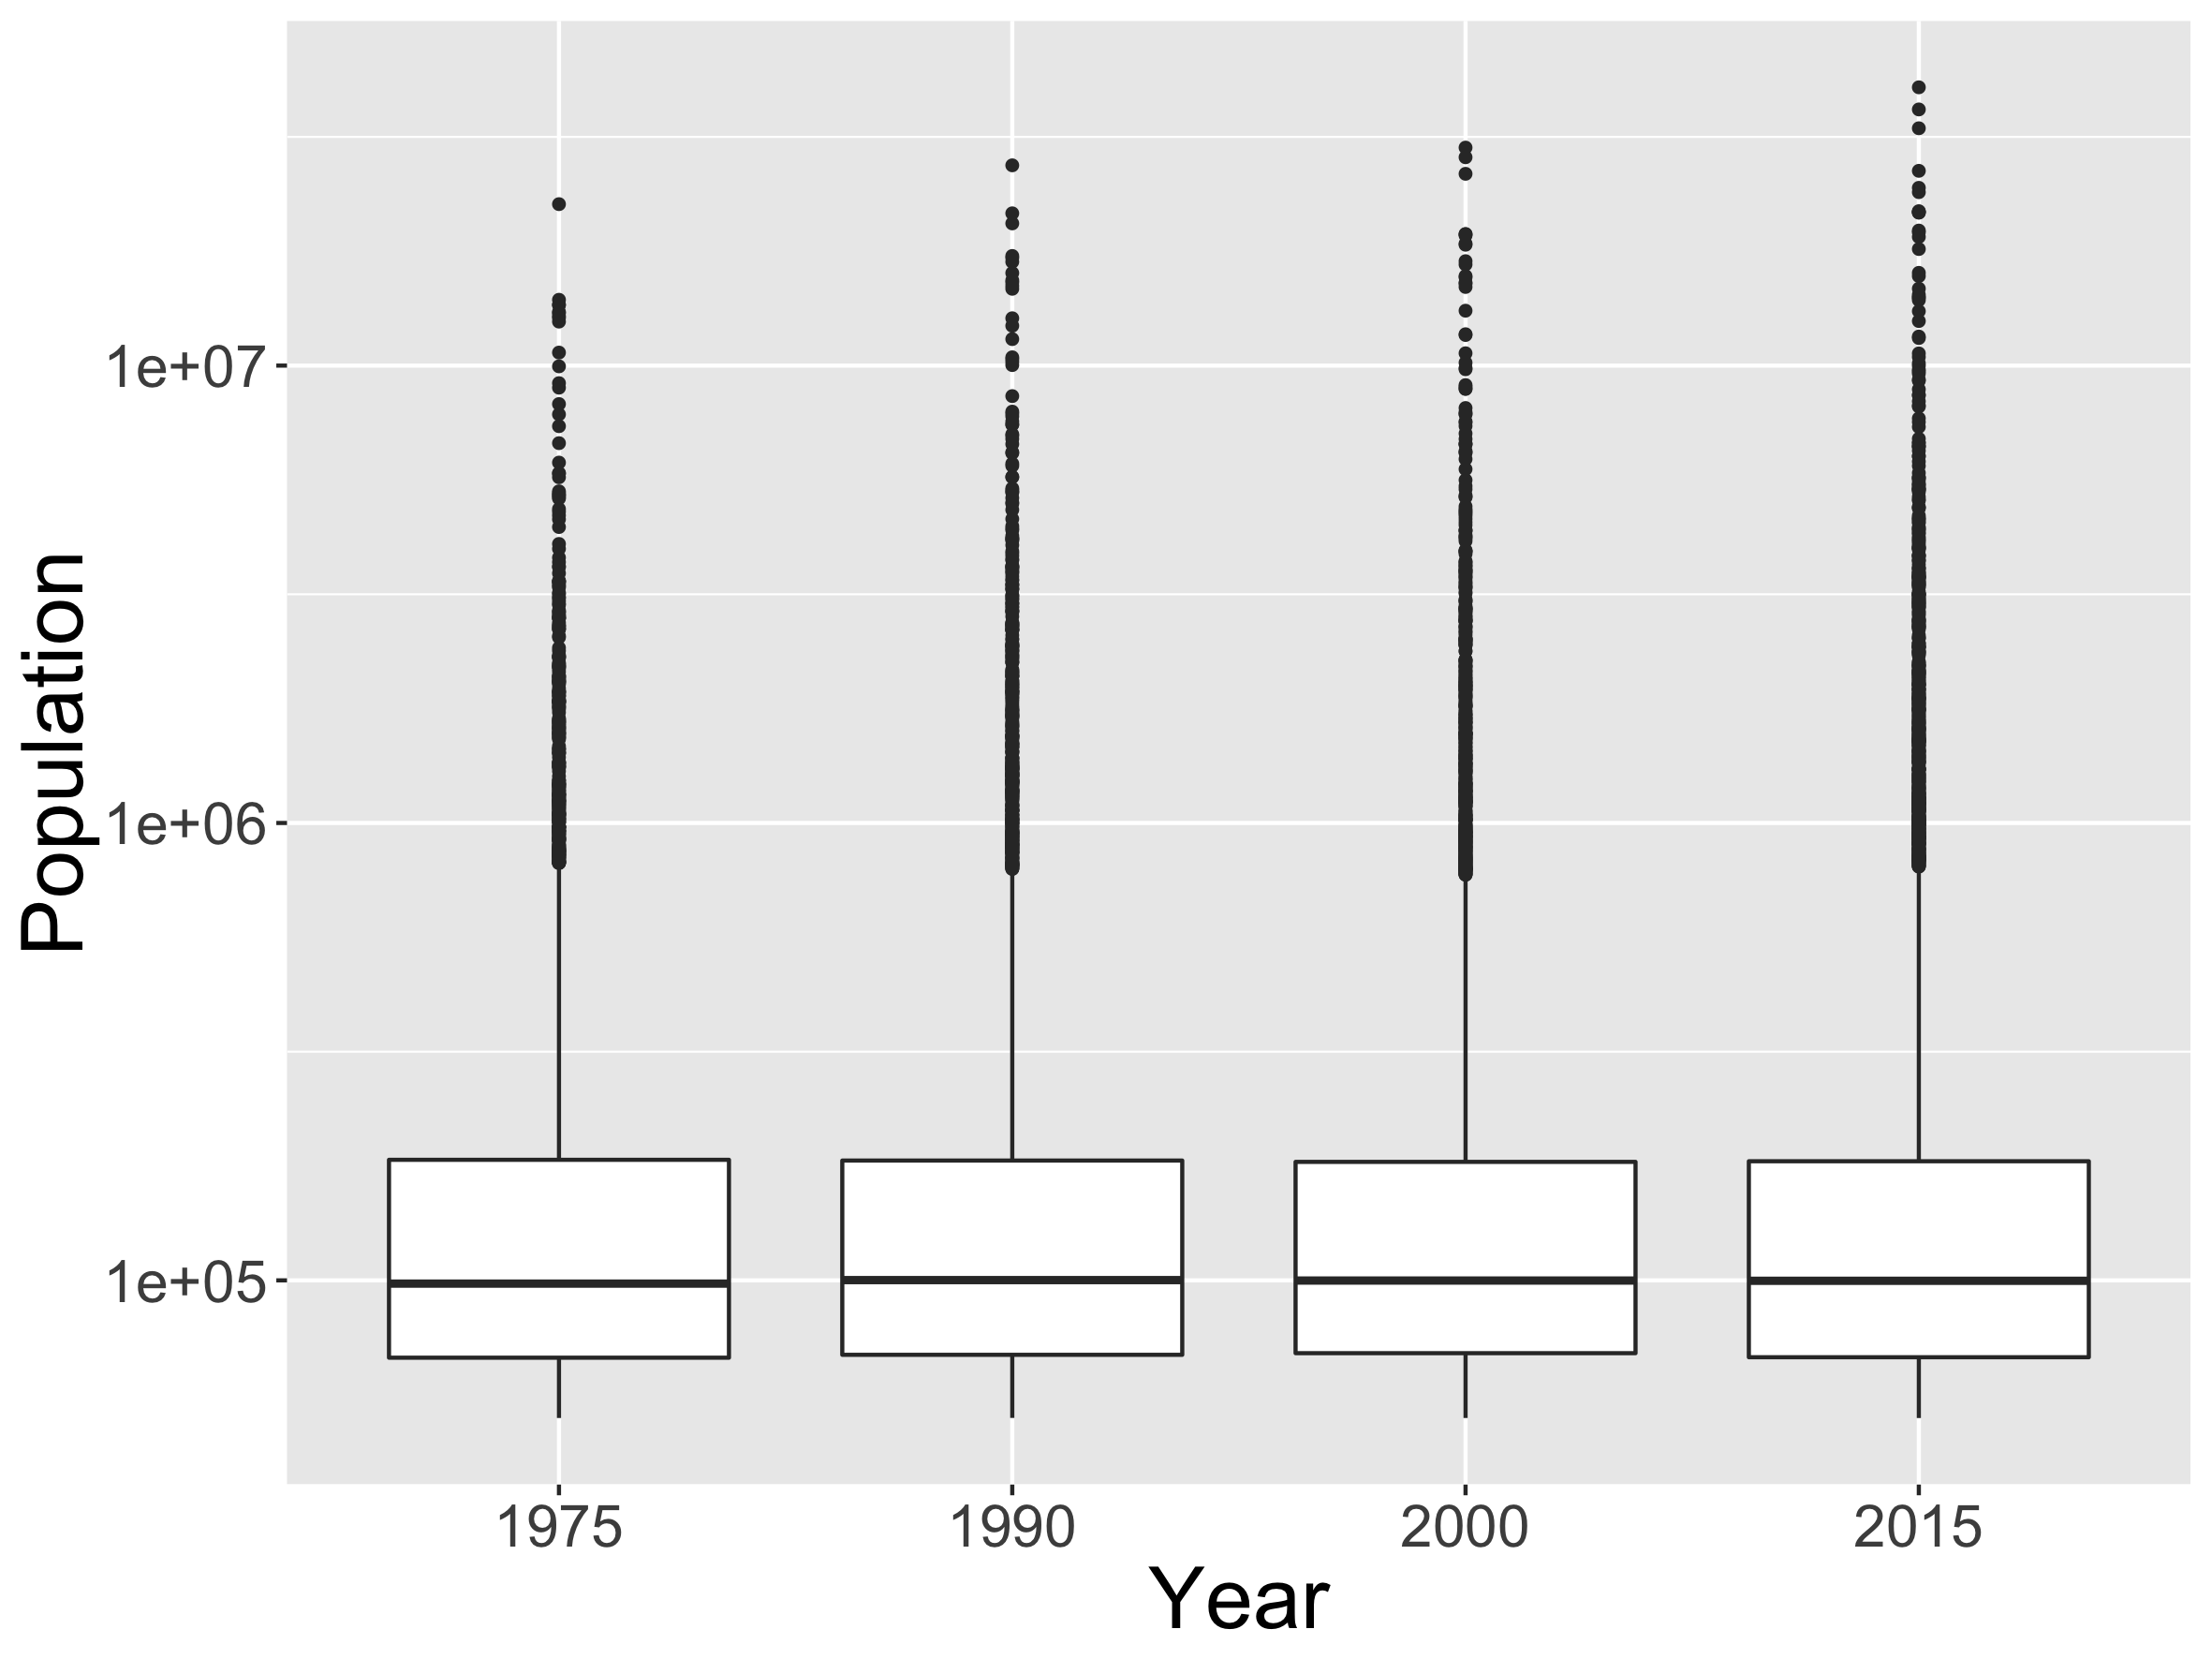
\includegraphics[width=0.8\textwidth]{figures/population_distributions.png}
\end{center}

}


\sframe{Urban systems summary}{
    
    % \cite{pumain2015multilevel} : number of cities / urban pop for each urban system
    % Summary table : number of cities, rank size slope, primacy index, total population
    
    % summary - 2015 - geodivercity urban systems

    \textit{Summary statistics in 2015 for urban systems studied in \cite{pumain2015multilevel}}
    
    \medskip
    
    \begin{center}
    \begin{tabular}{|c|c|c|c|c|c|}
    \hline
        System & Population & Cities & Primacy & Rank-size & R2  \\\hline
         Europe & 188Mio & 693 & 1.01 & $0.94 \pm 0.0026$ & 0.994  \\
         China & 567.2Mio & 1850 & 1.66 & $0.91 \pm 0.0011$ & 0.997  \\
         Brazil & 111.7Mio & 349 & 1.95 & $0.99 \pm 0.0026$ & 0.998  \\
         India & 703.1Mio & 3248 & 1.22 & $0.78 \pm 0.0009$ & 0.996  \\
         South Africa & 25.3Mio & 77 & 1.85 & $1.05 \pm 0.020$ & 0.974  \\
         US & 153Mio & 324 & 1.12 & $1.16 \pm 0.0054$ & 0.992  \\
         FSU & 120.3Mio & 450 & 3.27 & $0.92 \pm 0.0062$ & 0.979  \\\hline
    \end{tabular}
    \end{center}

}





\sframe{Urban systems hierarchy}{

Reproducing results of \cite{pumain2015multilevel} for large urban systems

% Brazil, China, US, Europe, South Africa, URSS, India

\begin{center}
    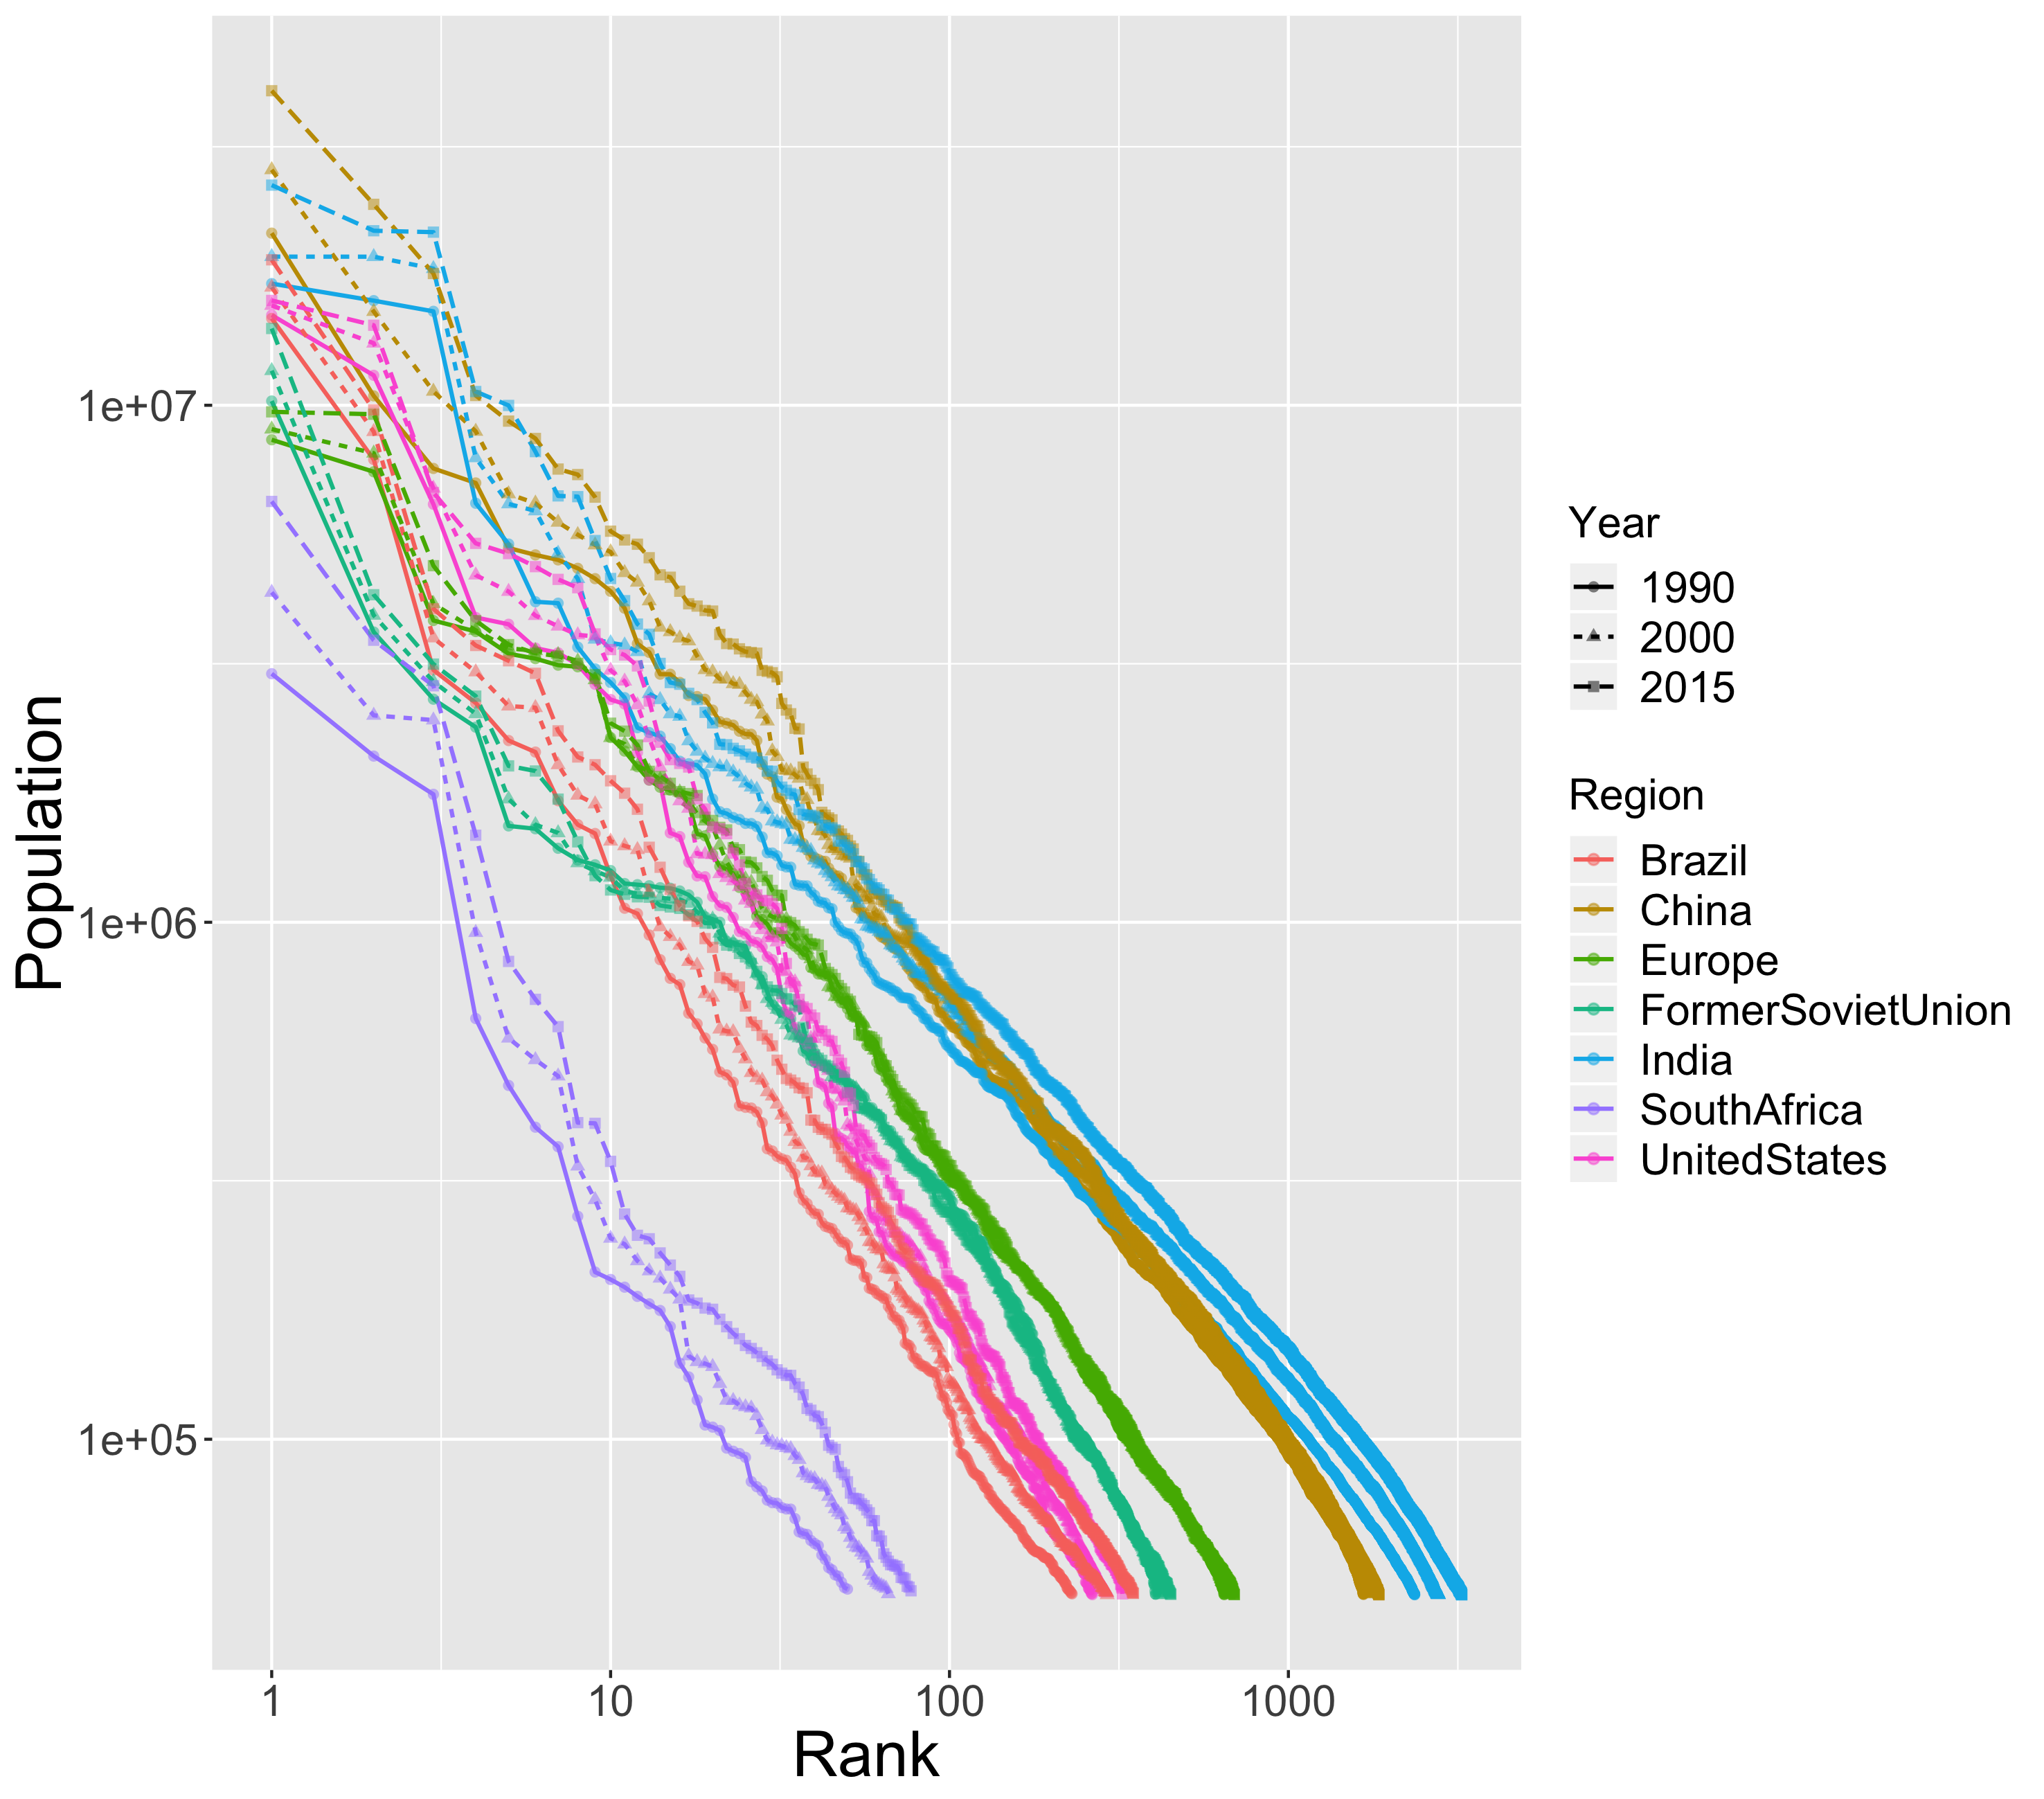
\includegraphics[height=0.8\textheight,width=0.8\textwidth]{figures/RankSize_Europe-China-Brazil-India-SouthAfrica-UnitedStates-FormerSovietUnion_years-90-00-15.png}
\end{center}


}


\sframe{Correlations between urban indicators}{

% includes test of gibrat law : correlation pops / growth rates

\begin{center}
    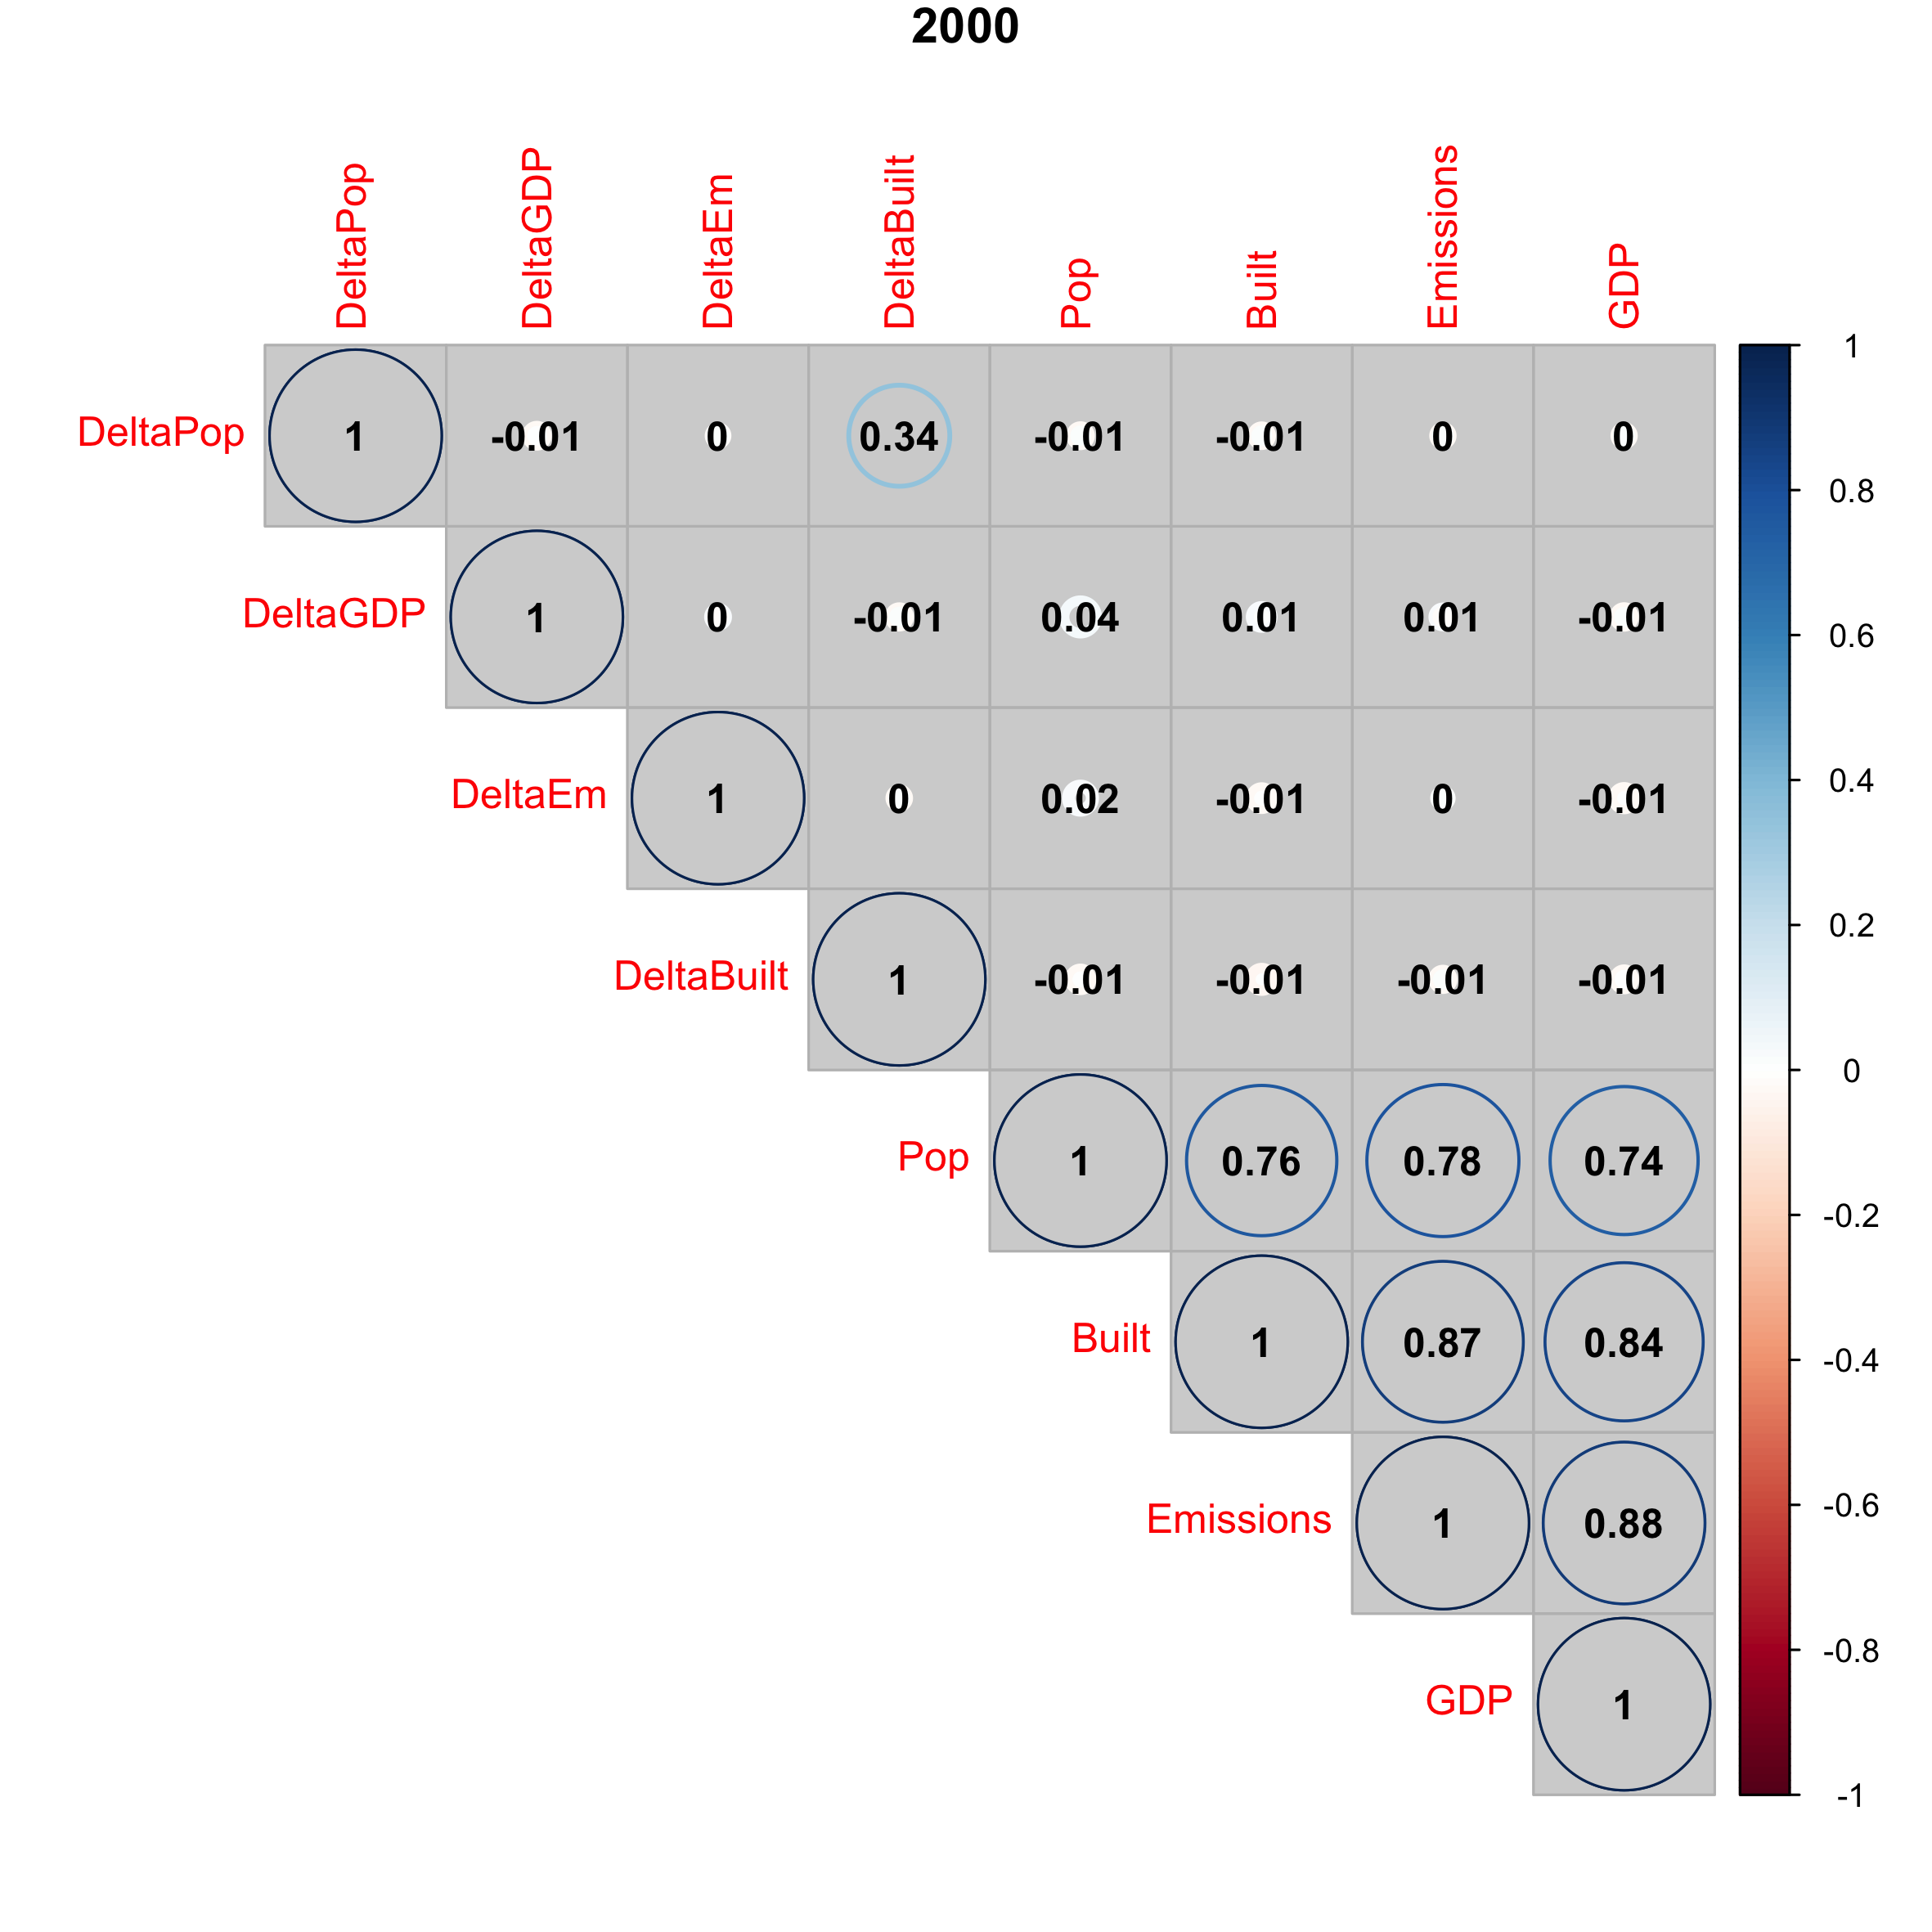
\includegraphics[width=0.46\textwidth]{figures/correlations_00.png}\hspace{0.2cm}
    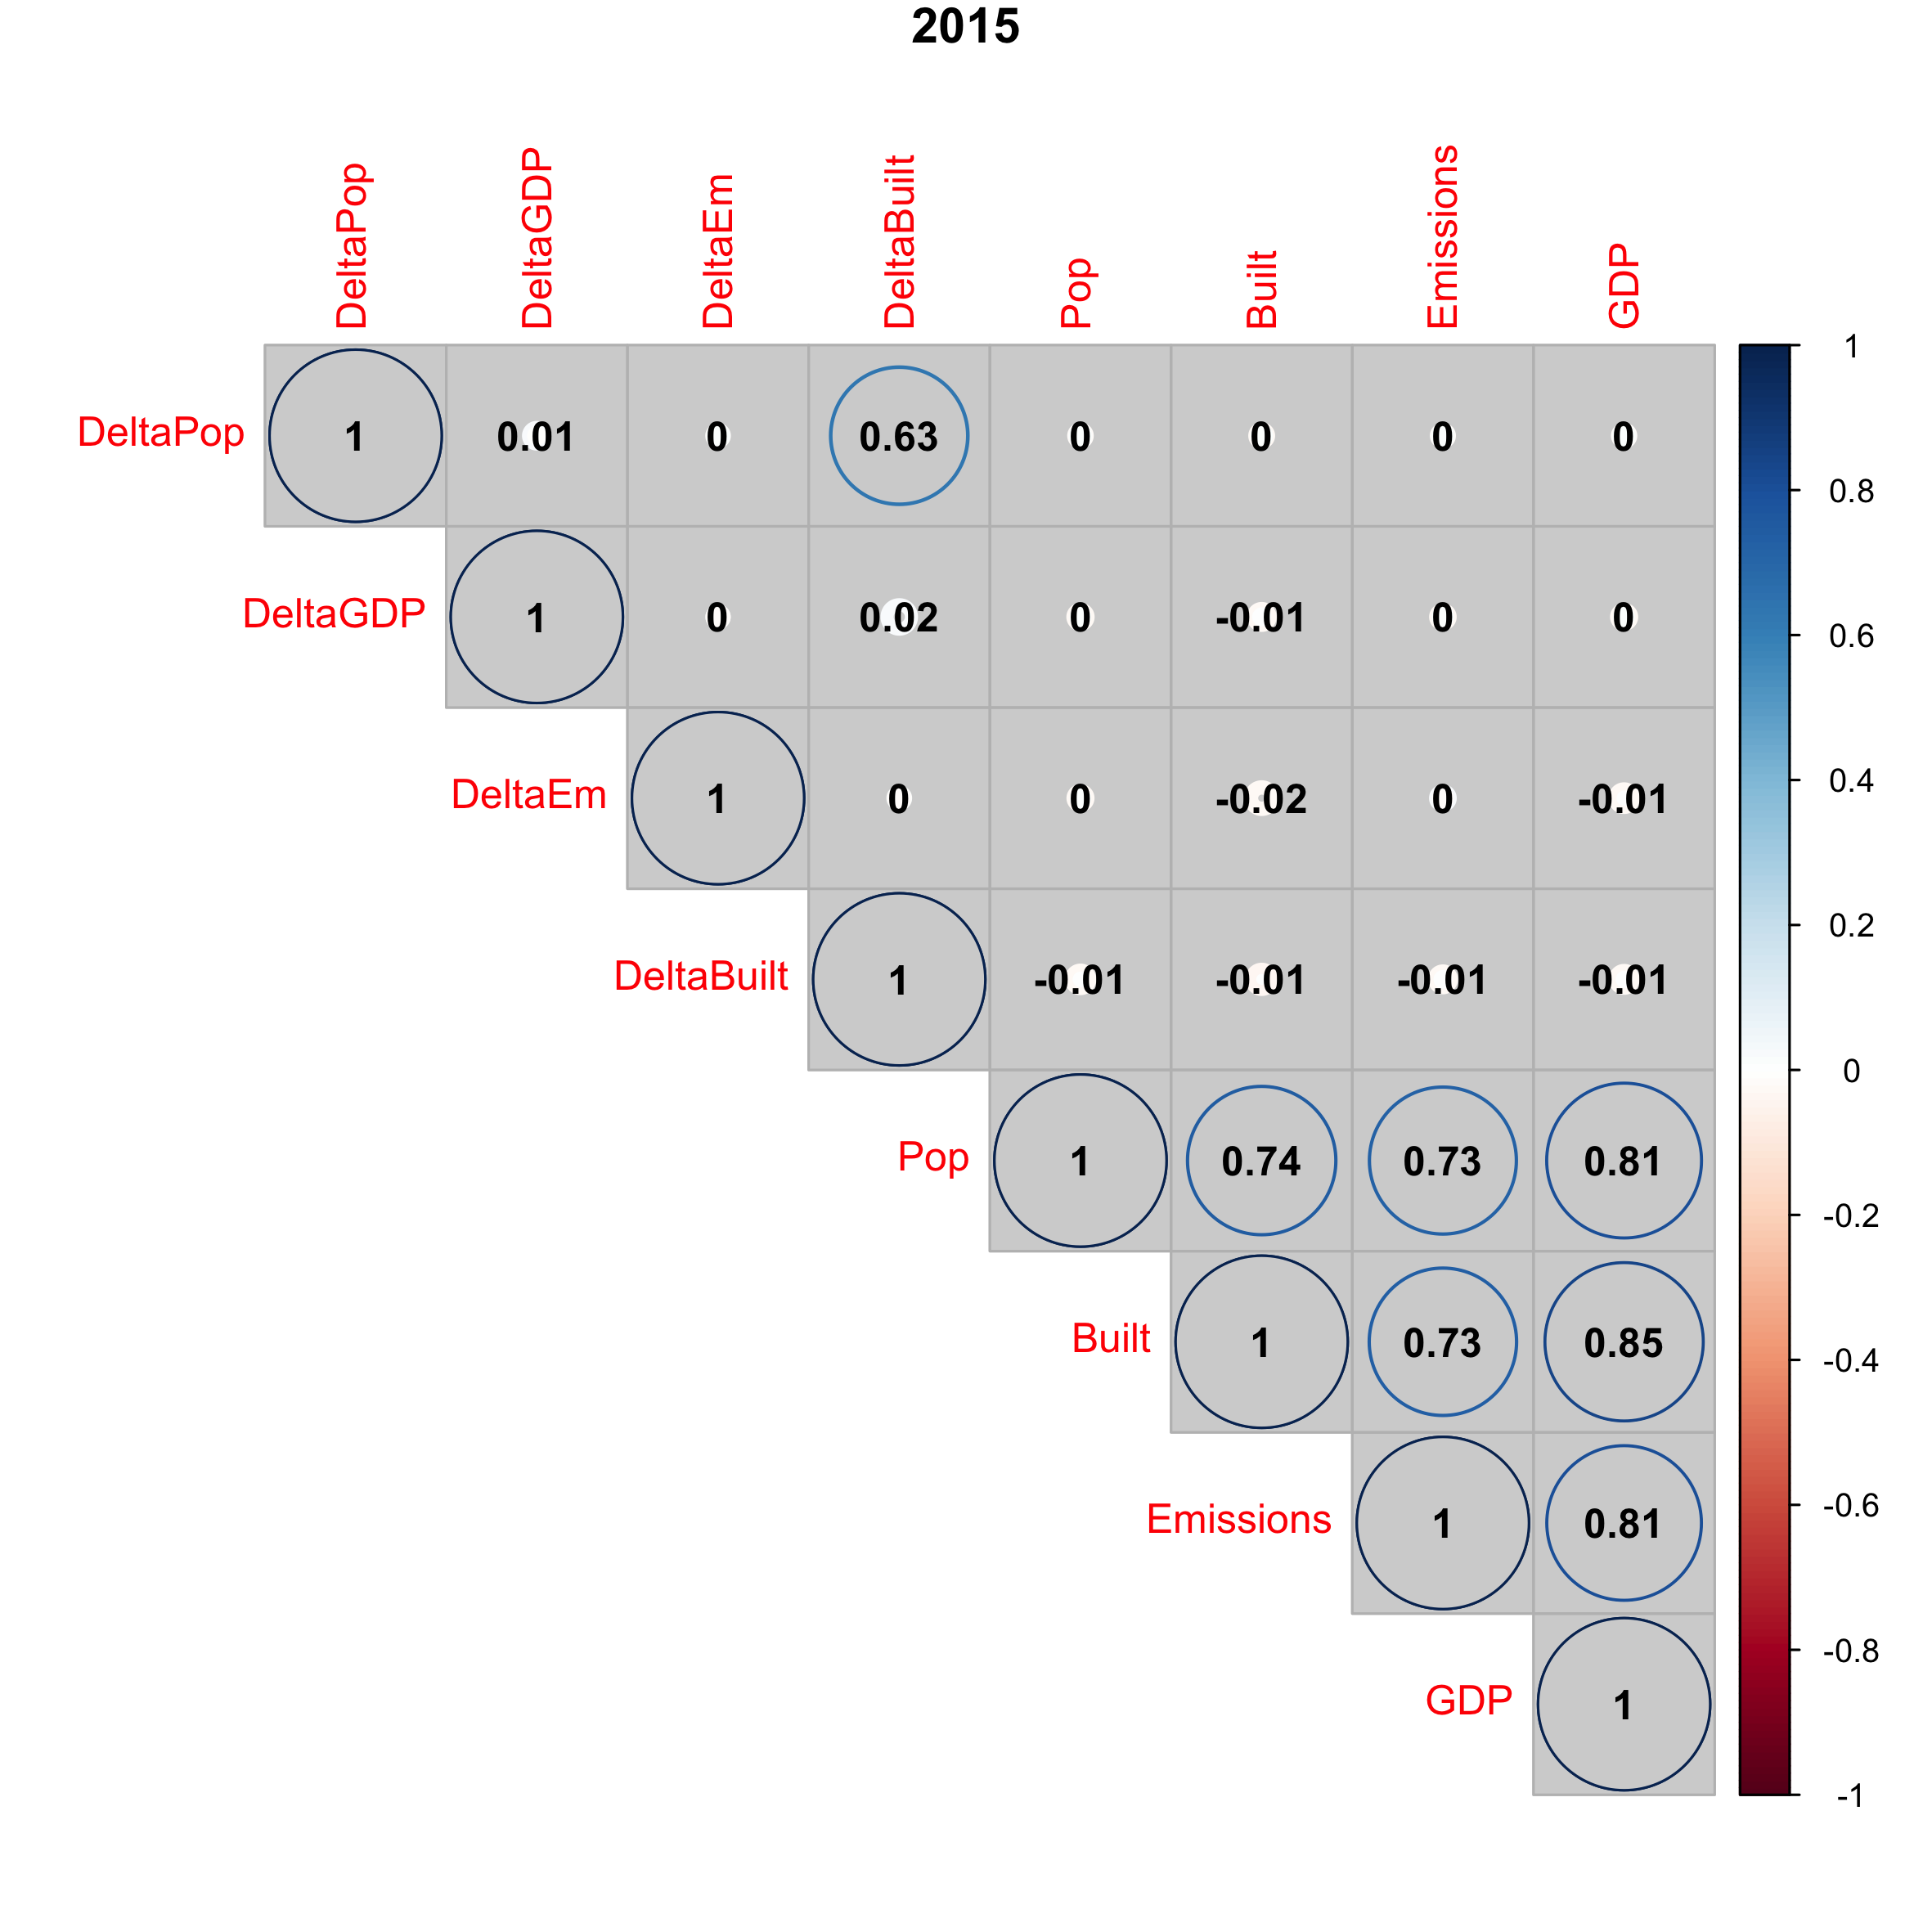
\includegraphics[width=0.46\textwidth]{figures/correlations_15.png}
\end{center}



}

\sframe{Scaling laws}{

Generalizing existing studies

\begin{center}
    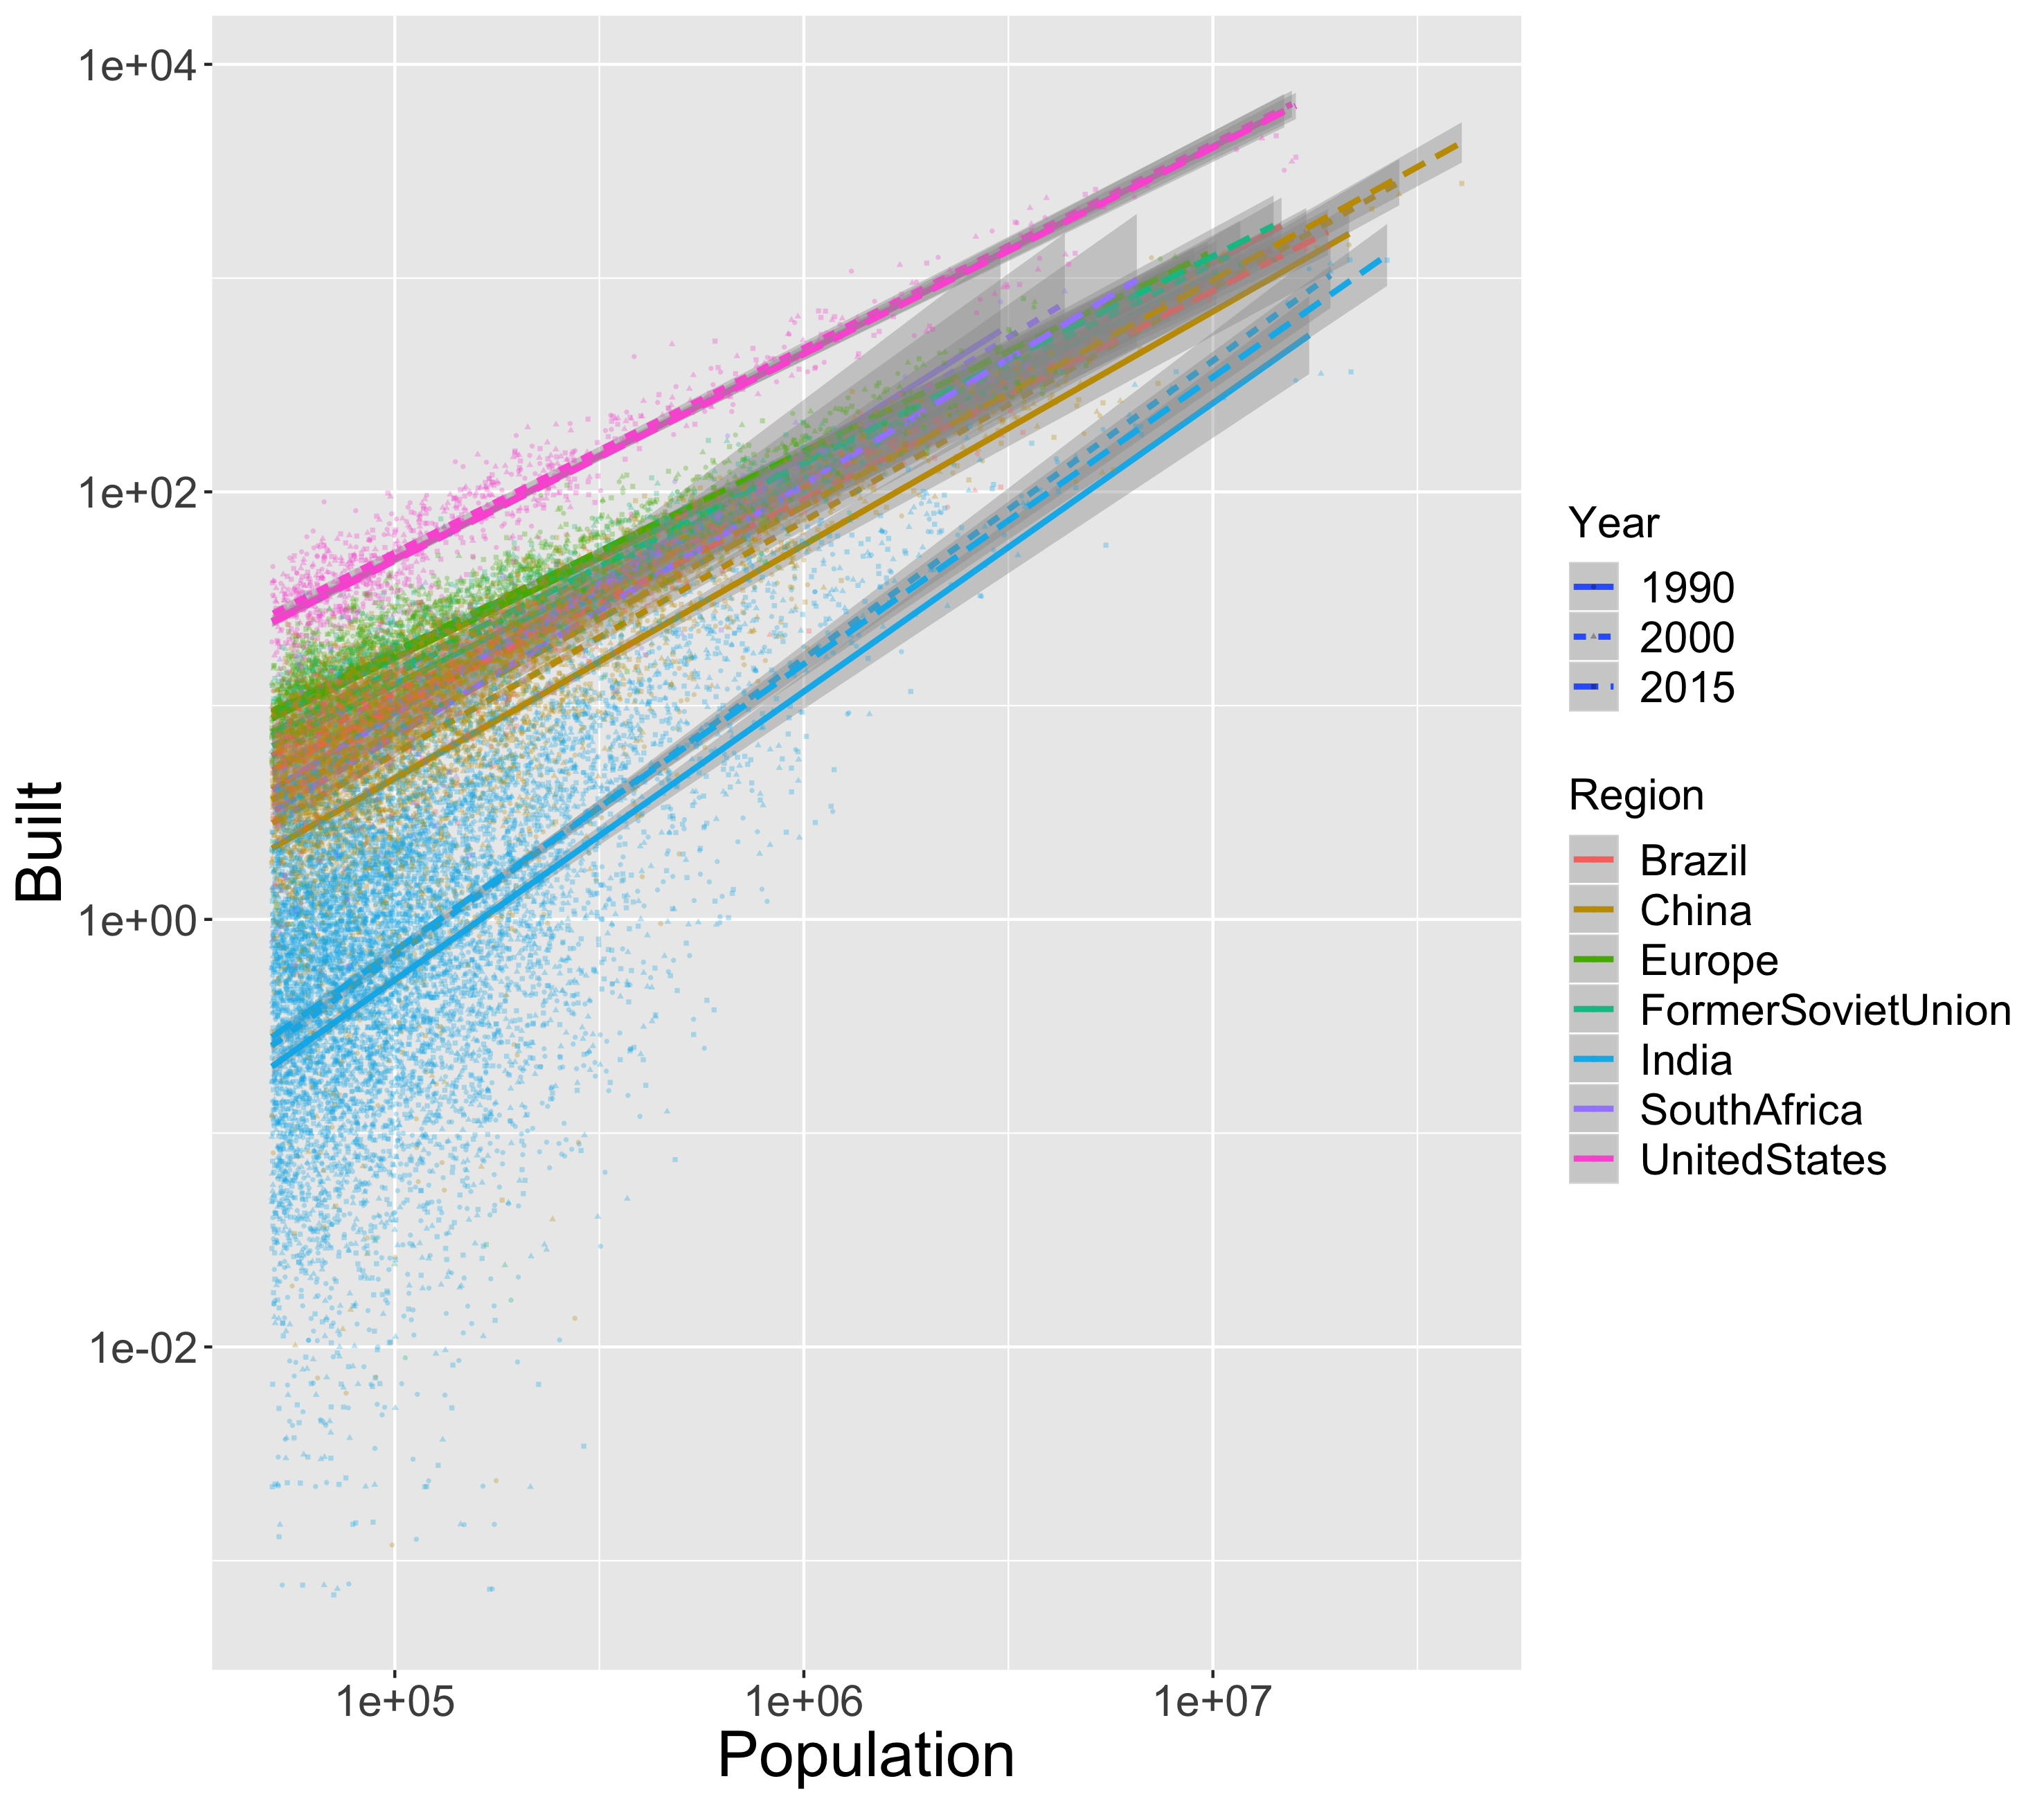
\includegraphics[width=0.32\textwidth]{figures/Built-fitted_Europe-China-Brazil-India-SouthAfrica-UnitedStates-FormerSovietUnion_years-90-00-15.png}
    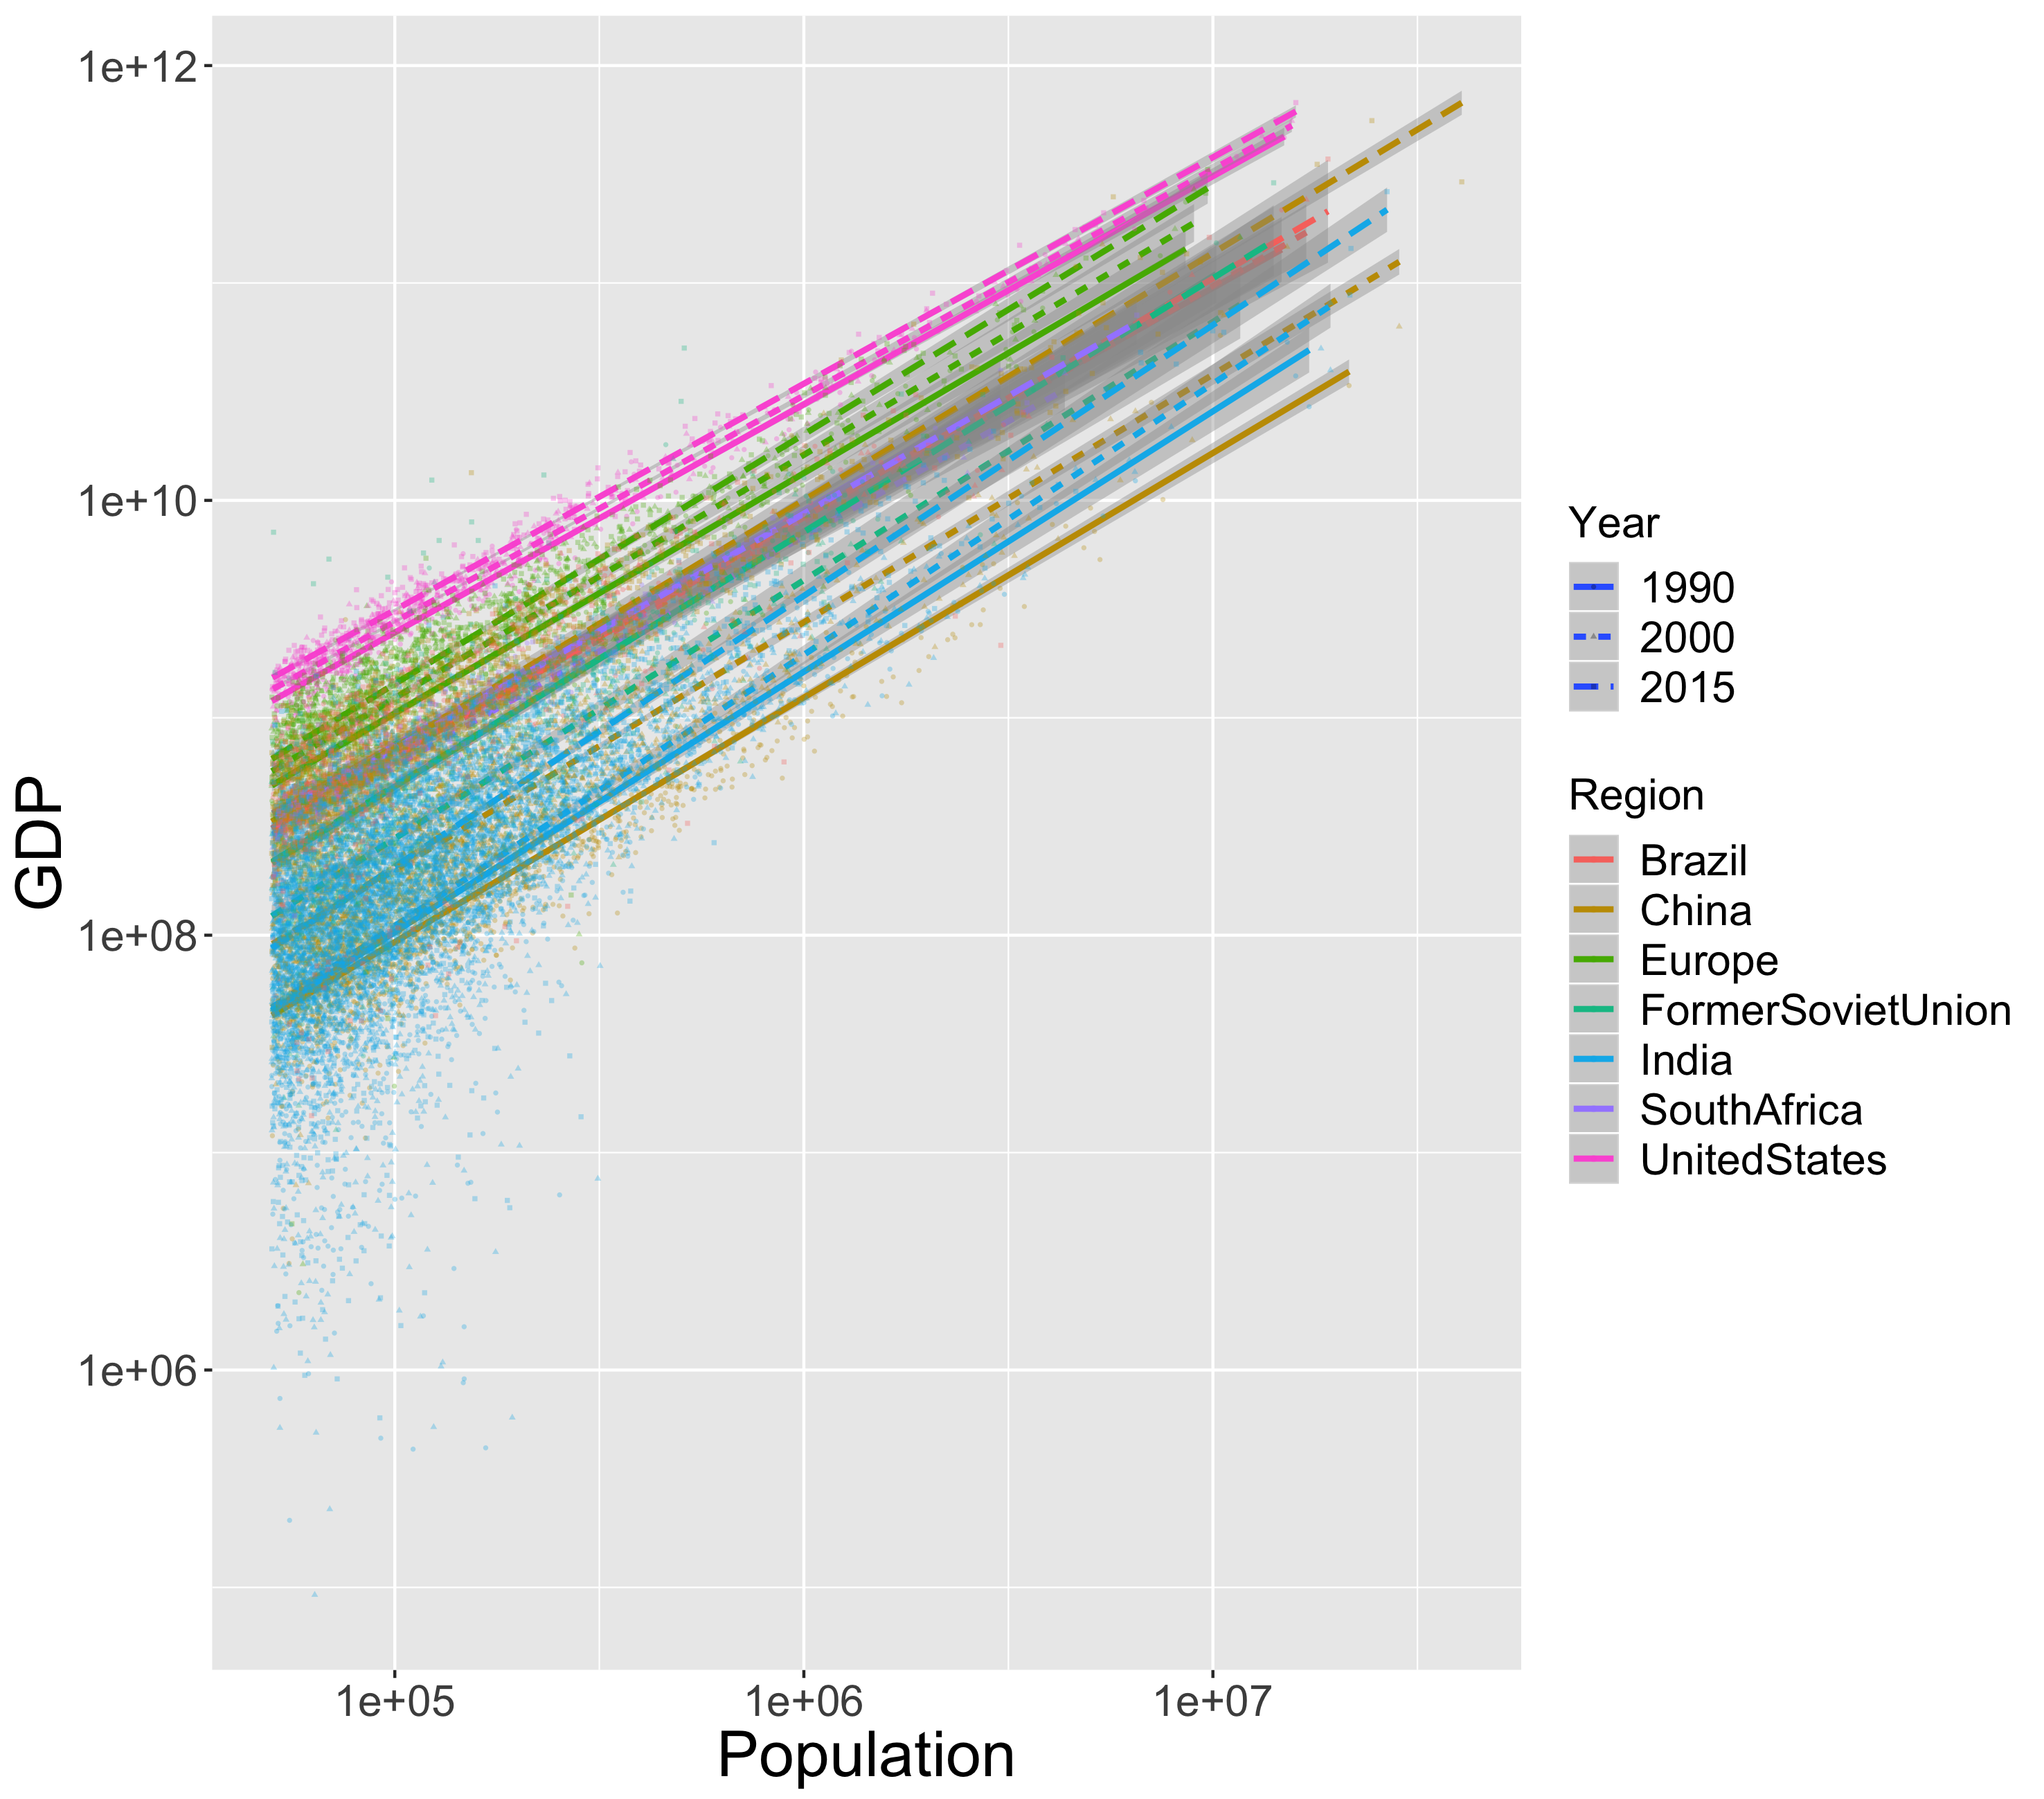
\includegraphics[width=0.32\textwidth]{figures/GDP-fitted_Europe-China-Brazil-India-SouthAfrica-UnitedStates-FormerSovietUnion_years-90-00-15.png}
    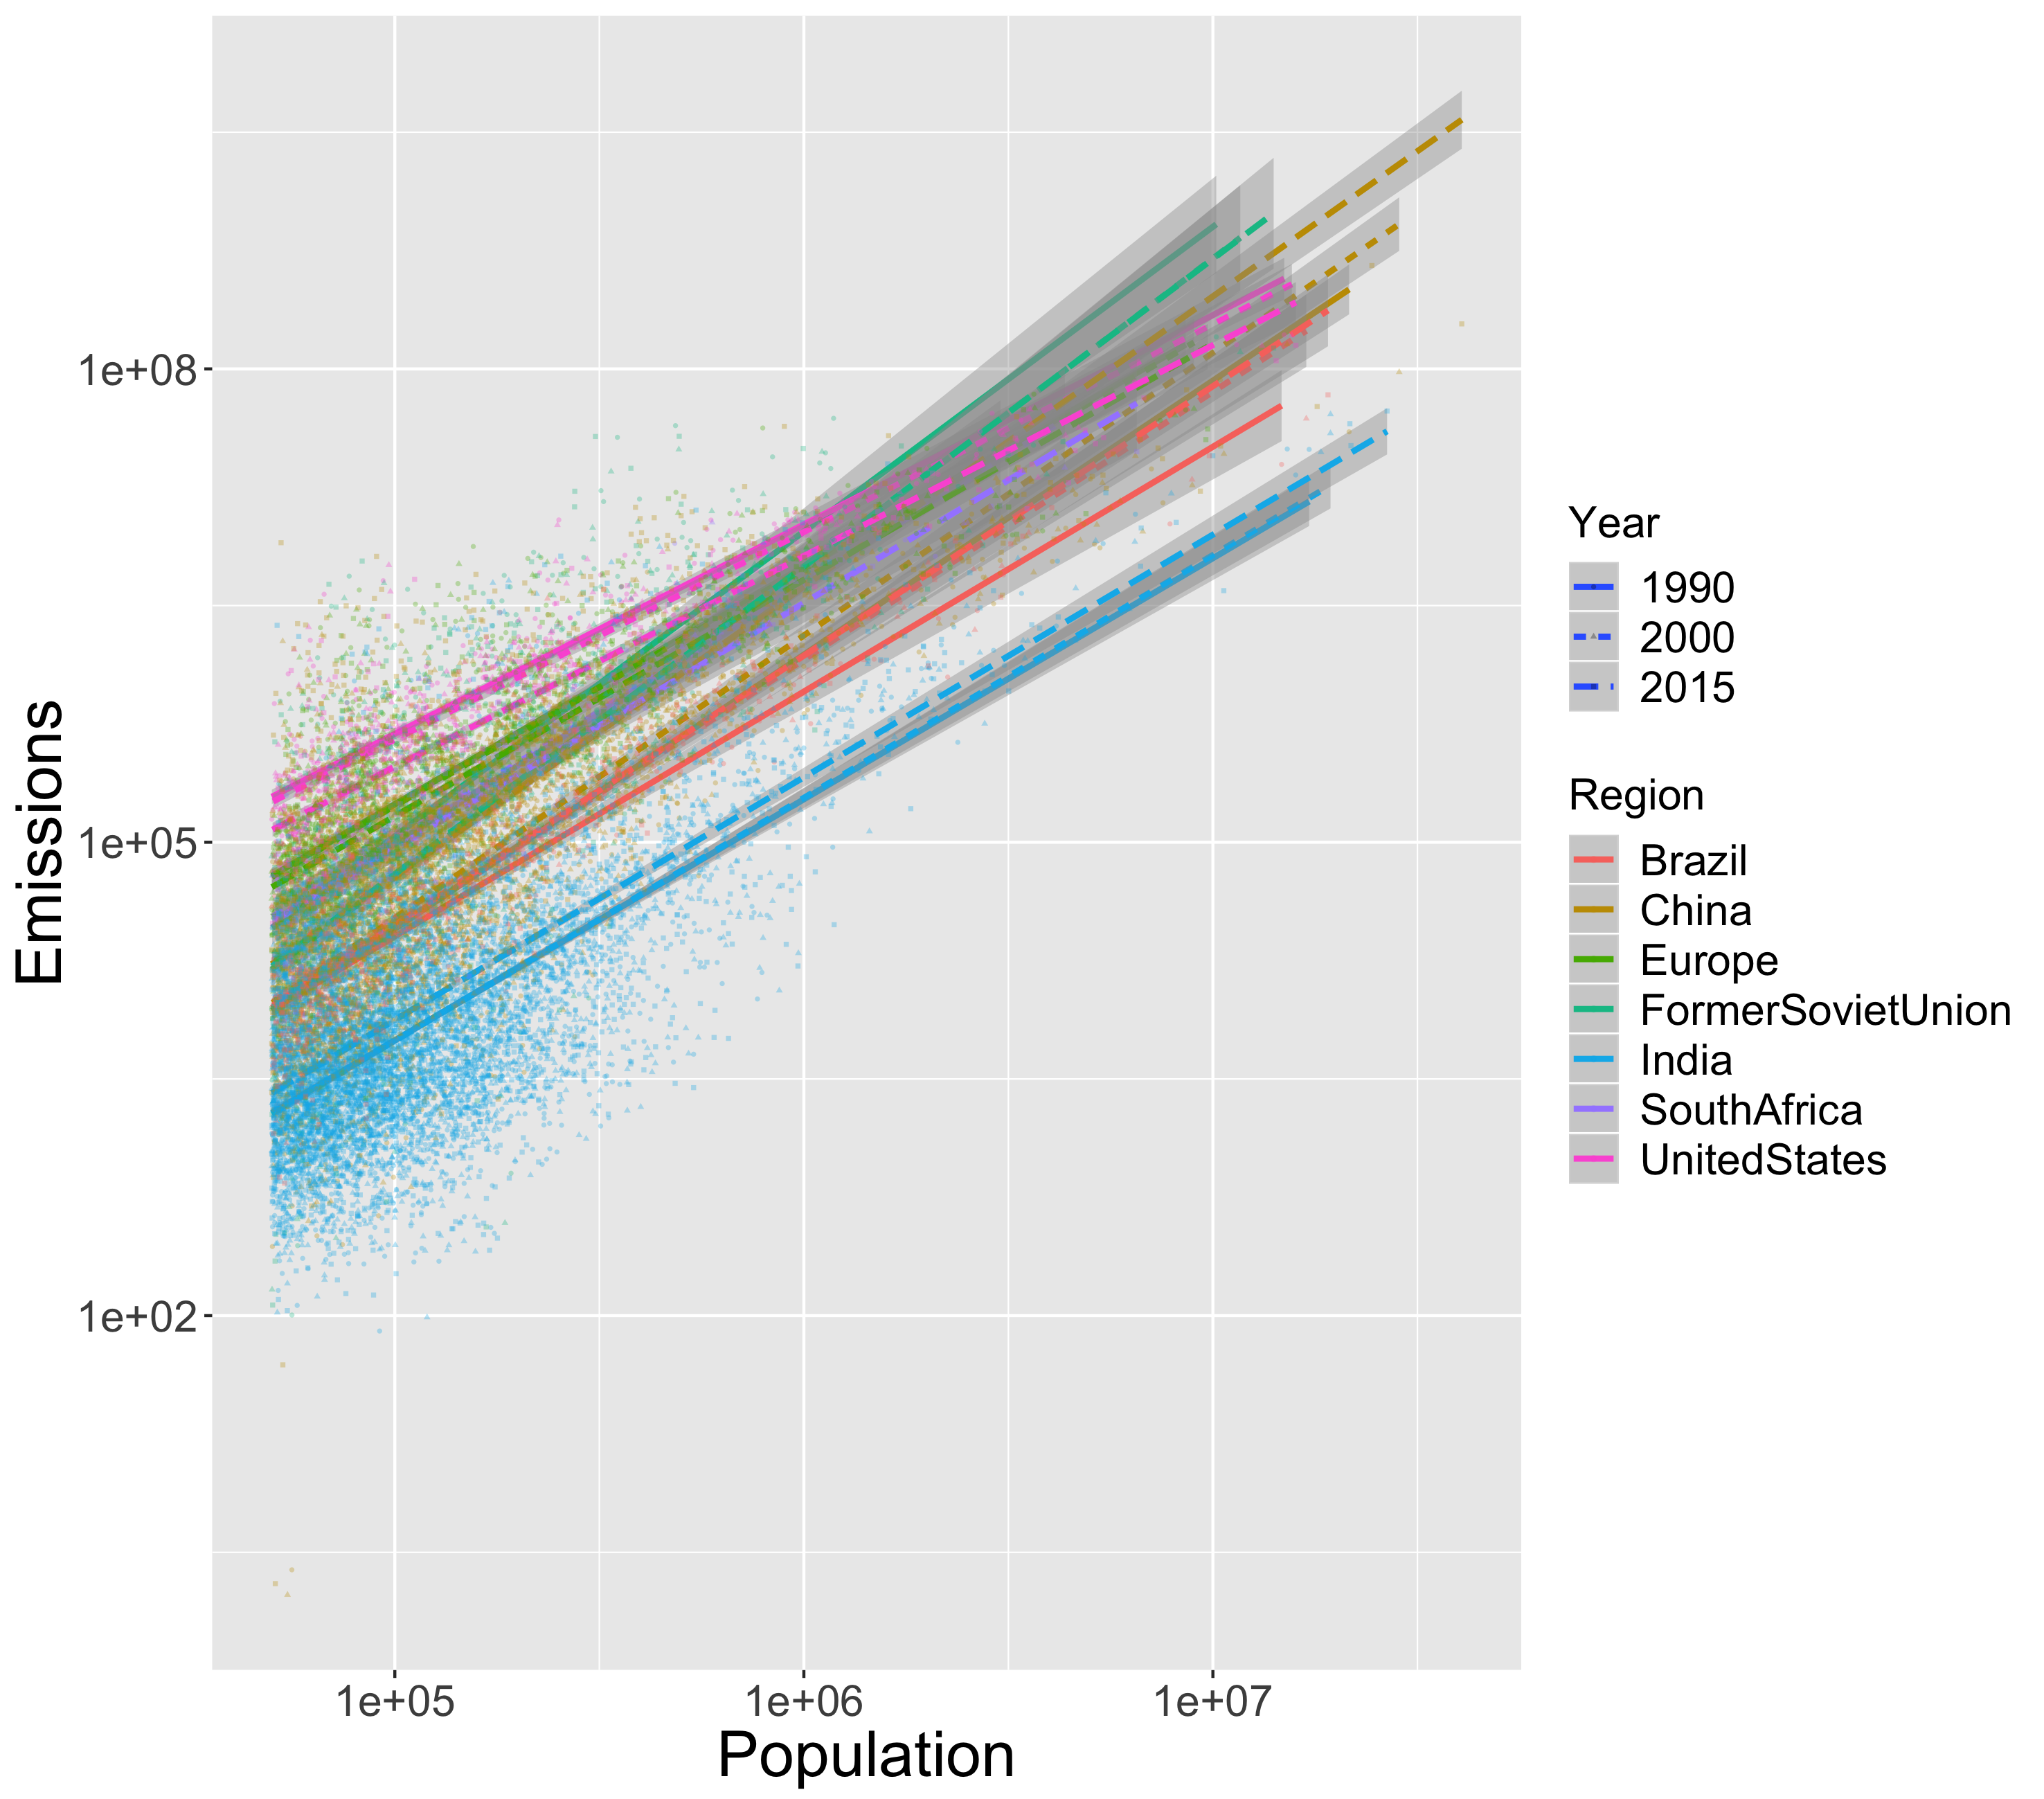
\includegraphics[width=0.32\textwidth]{figures/Emissions-fitted_Europe-China-Brazil-India-SouthAfrica-UnitedStates-FormerSovietUnion_years-90-00-15.png}
\end{center}

}

\sframe{Evolution of scaling exponents}{

% evolution of scaling exponents in time

\textit{All indicators are stable in their confidence range}

\medskip

\begin{center}
    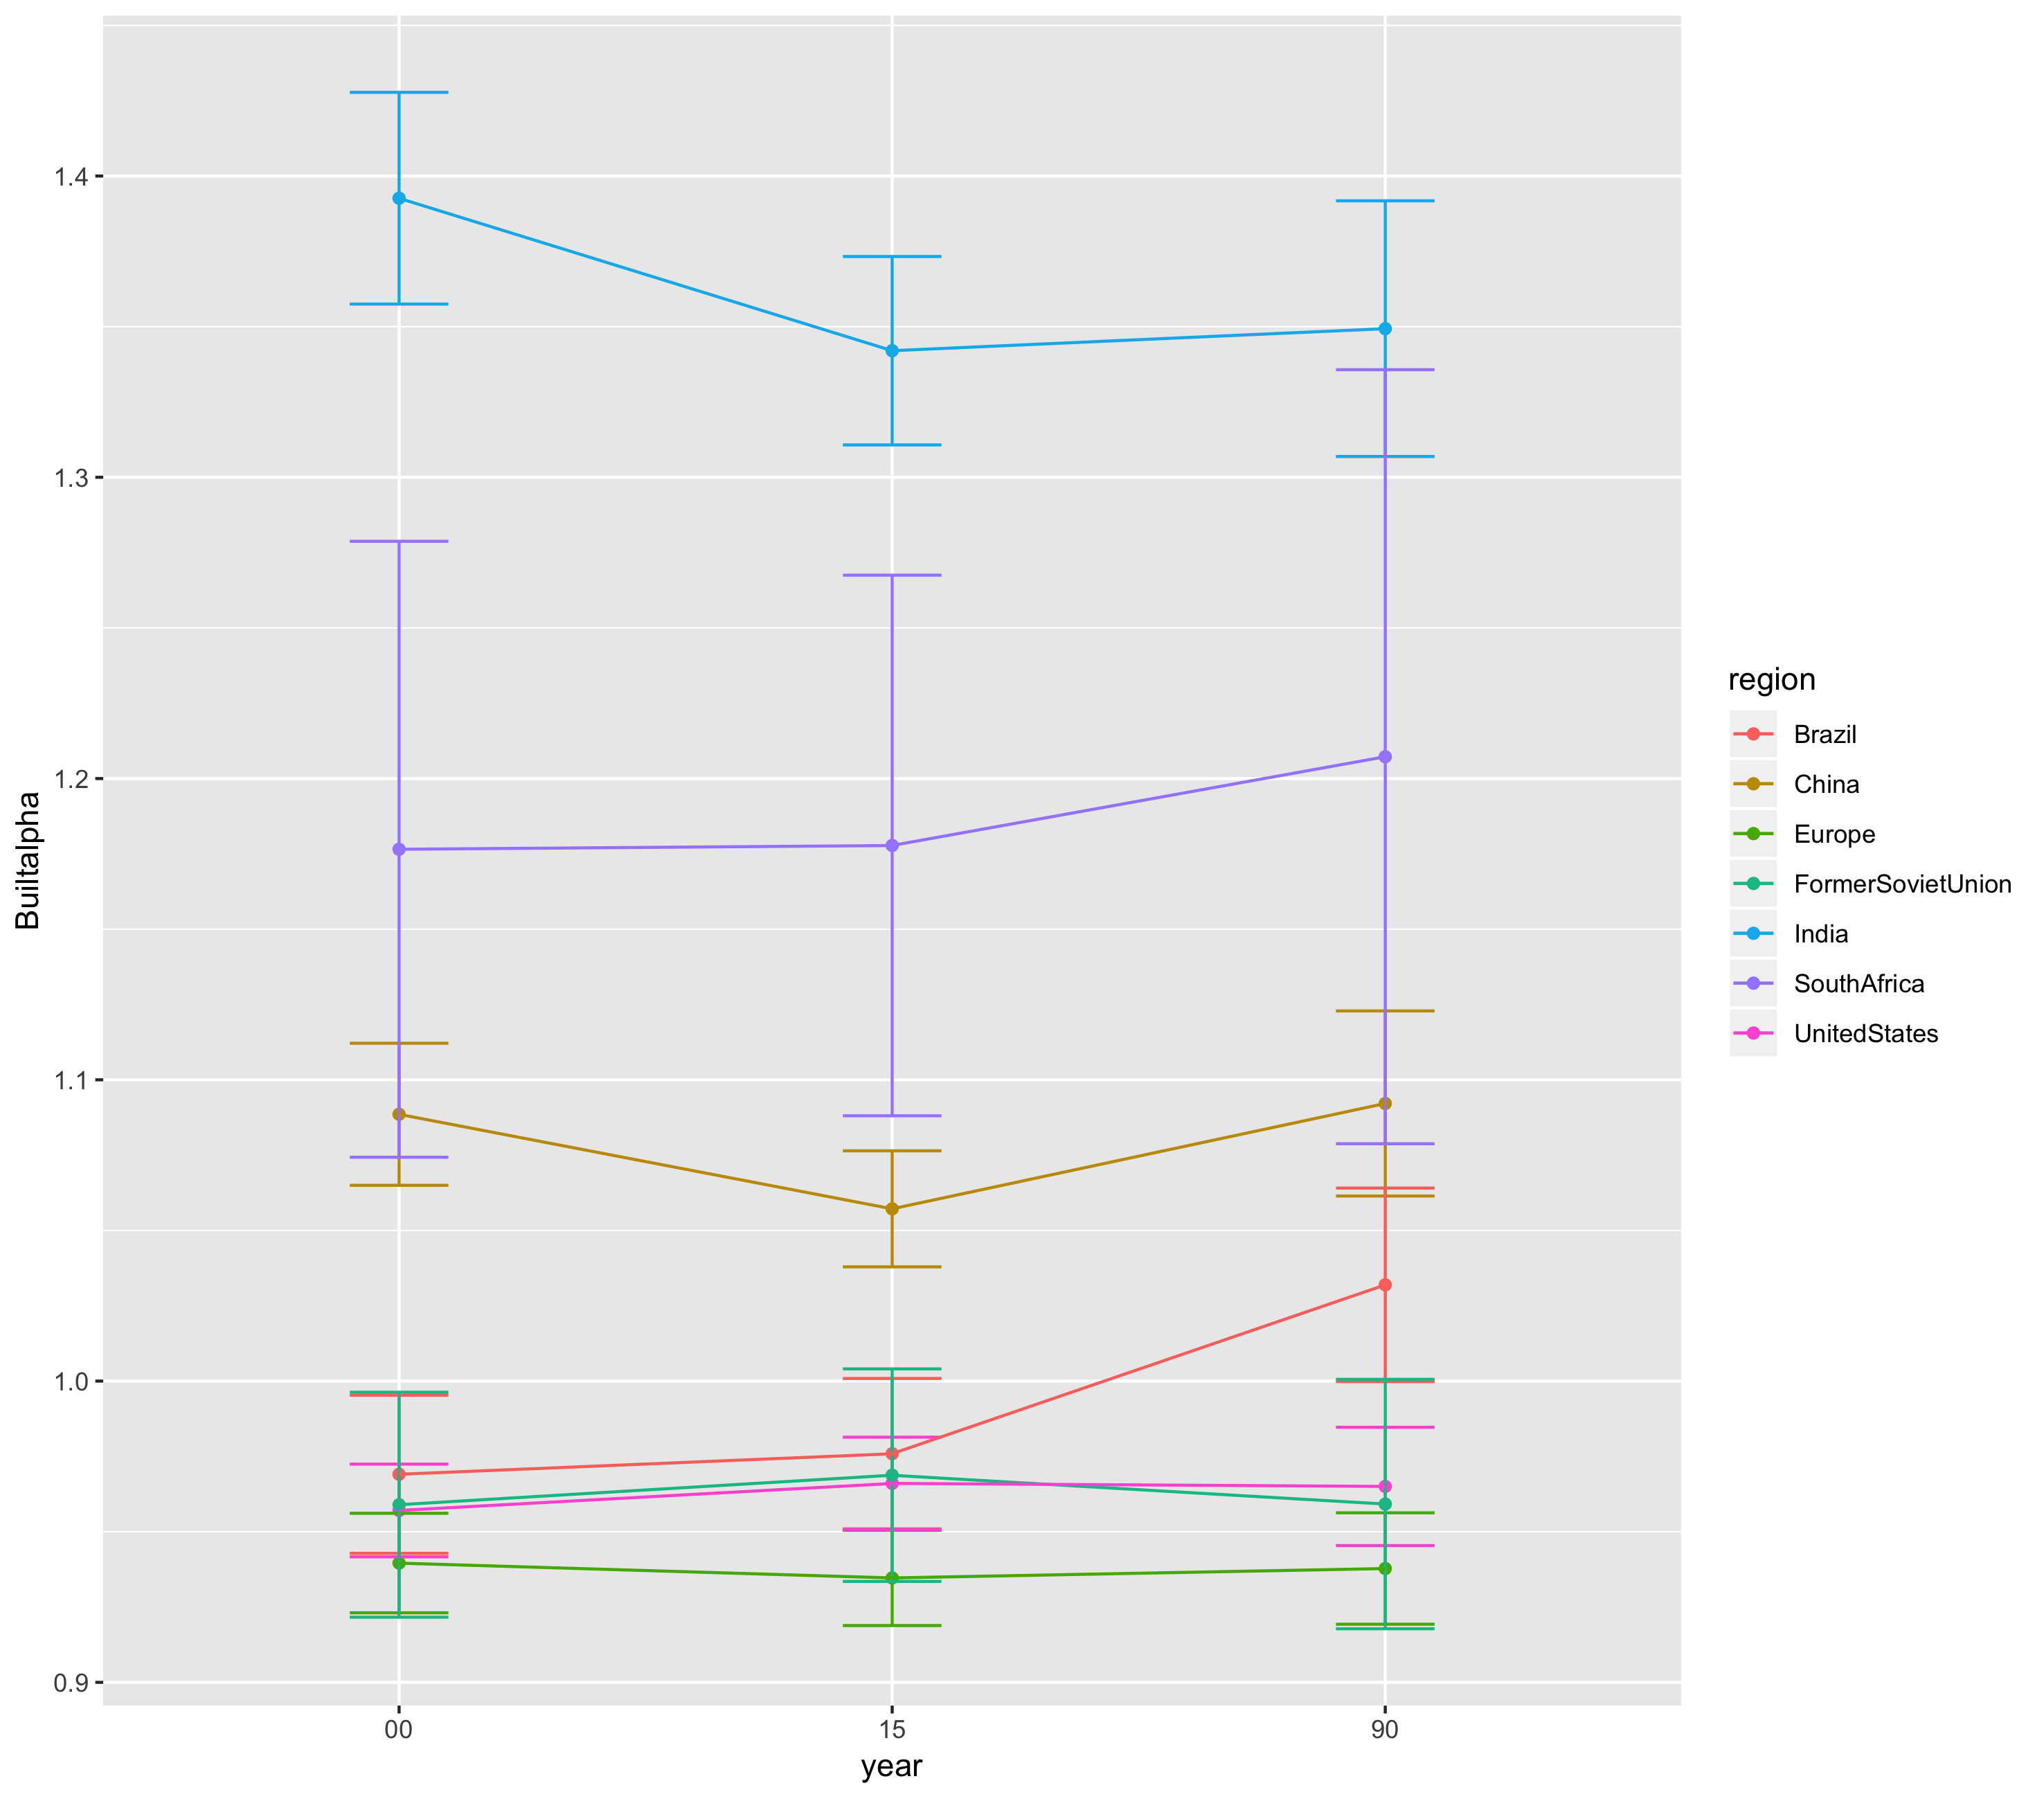
\includegraphics[width=0.32\textwidth,height=0.45\textheight]{figures/Built-evolution_Europe-China-Brazil-India-SouthAfrica-UnitedStates-FormerSovietUnion_years-90-00-15.png}
    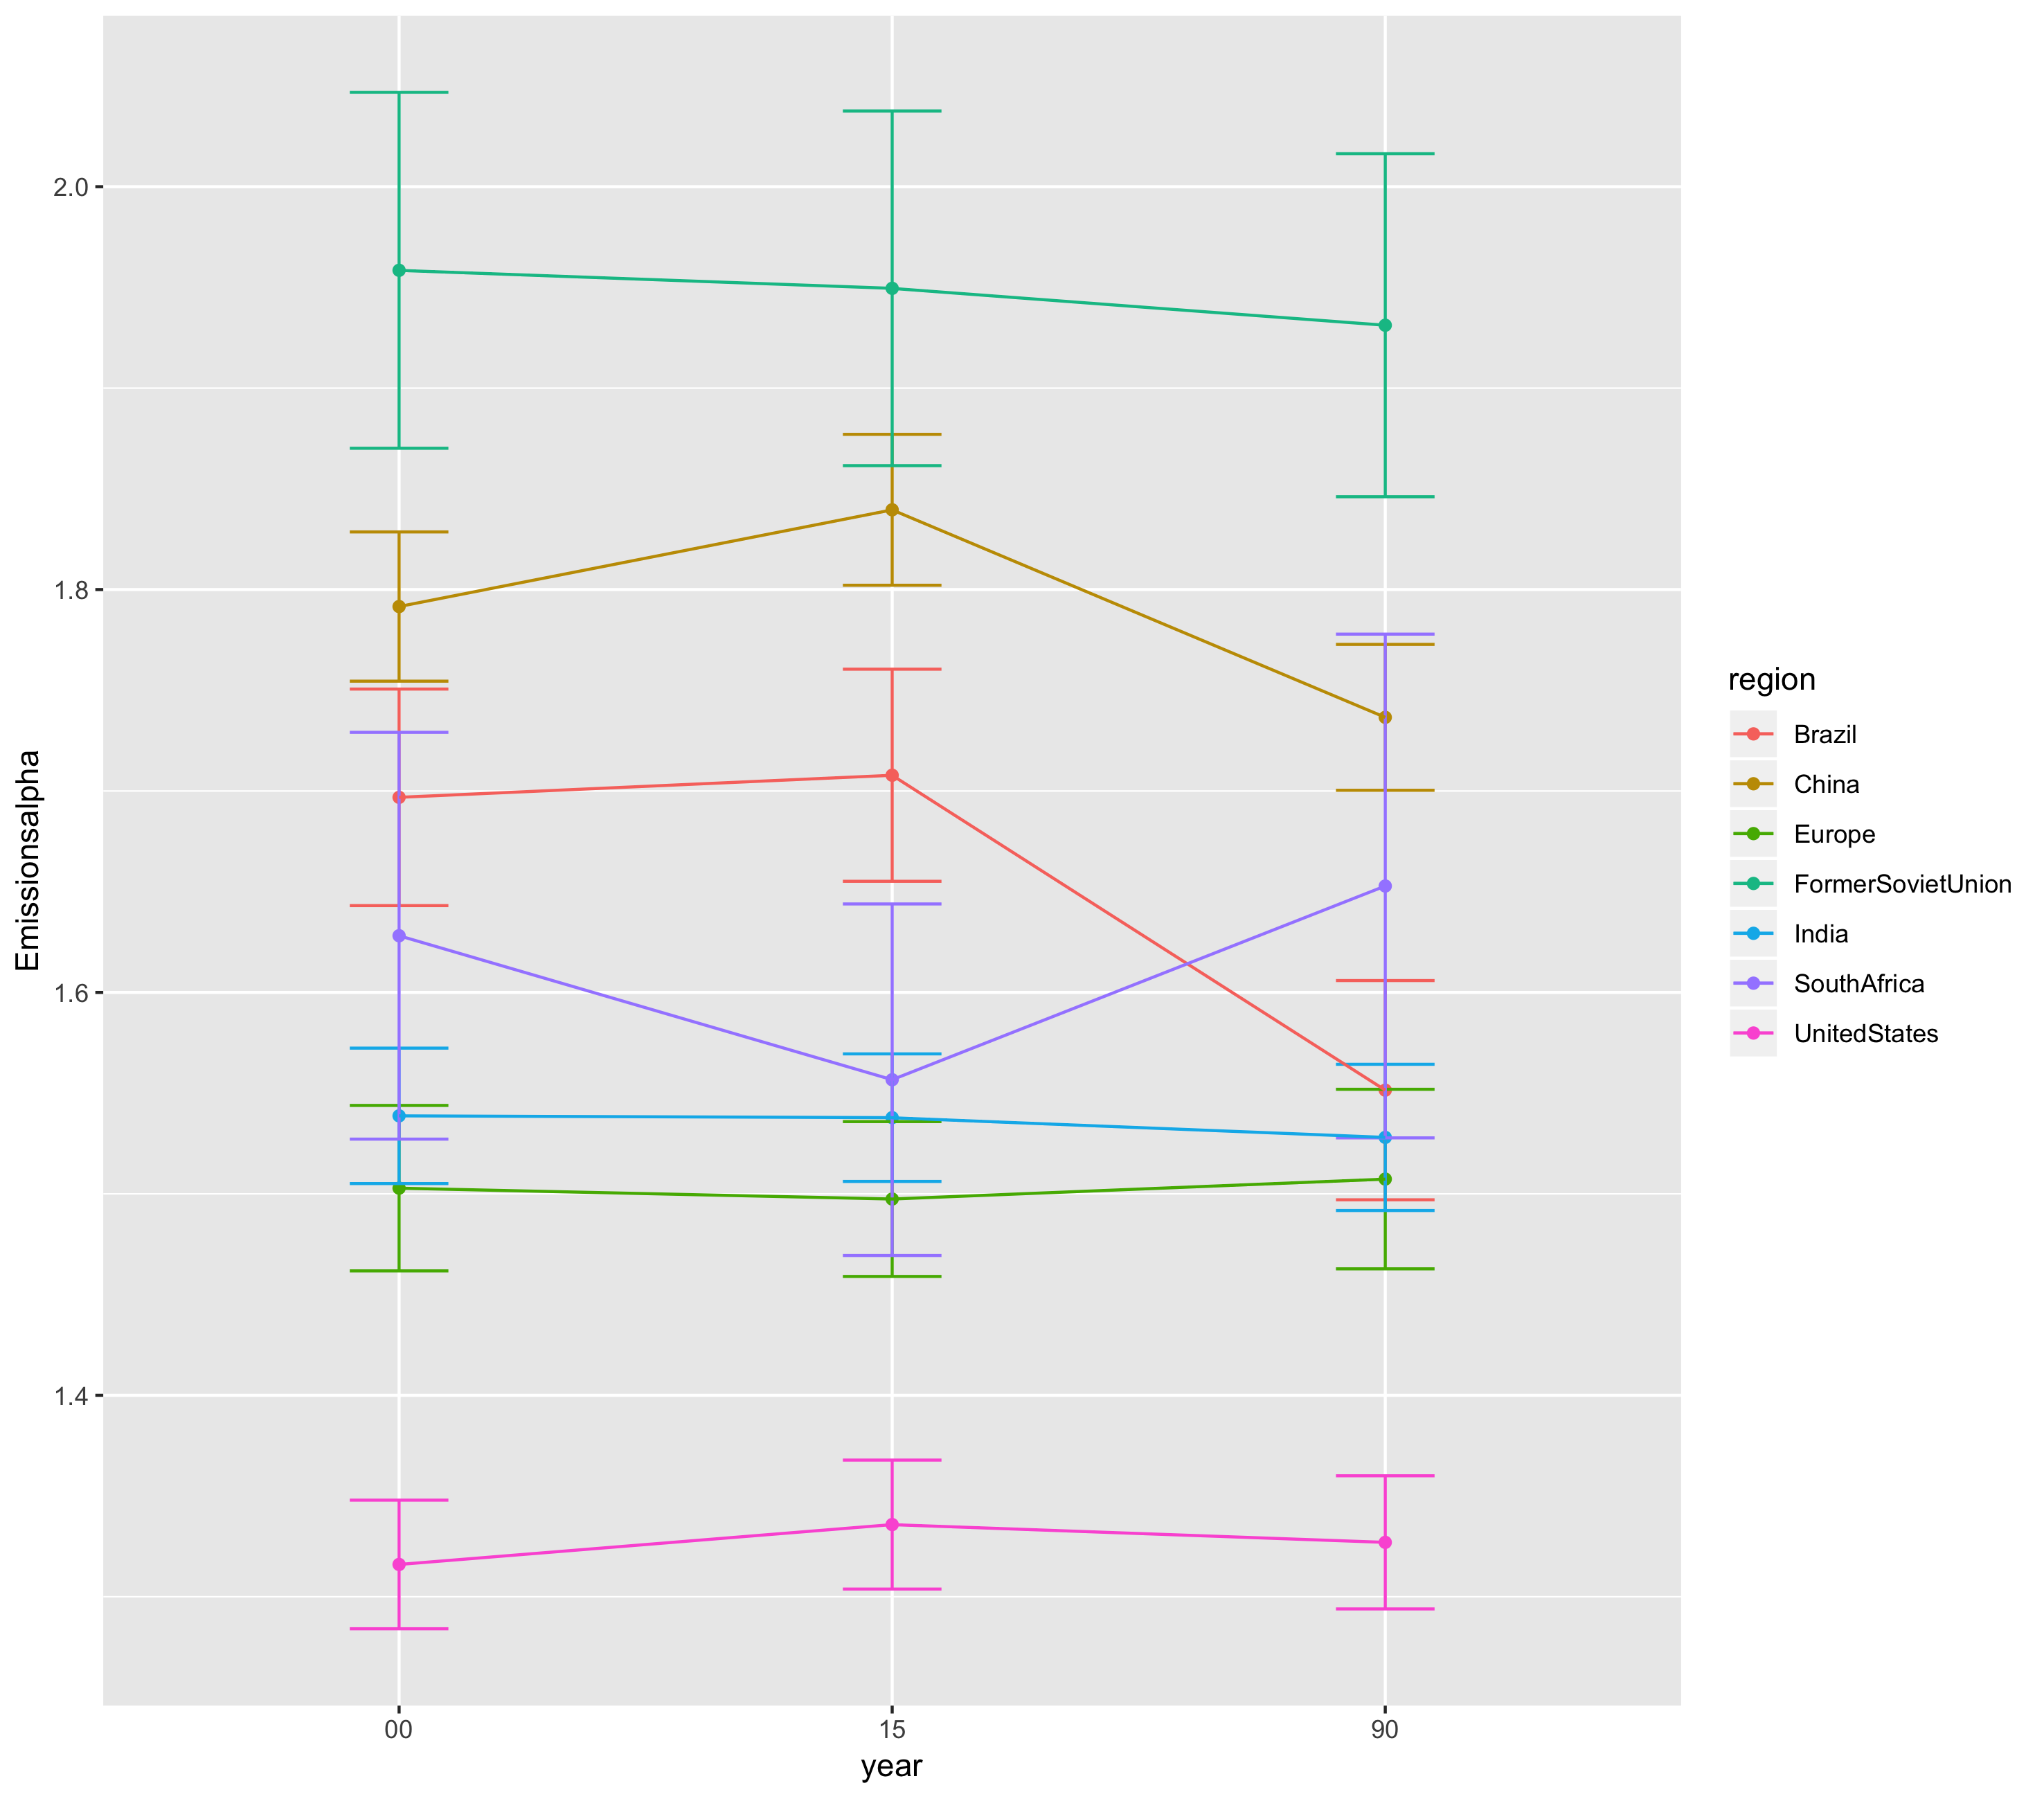
\includegraphics[width=0.32\textwidth,height=0.45\textheight]{figures/Emissions-evolution_Europe-China-Brazil-India-SouthAfrica-UnitedStates-FormerSovietUnion_years-90-00-15.png}
    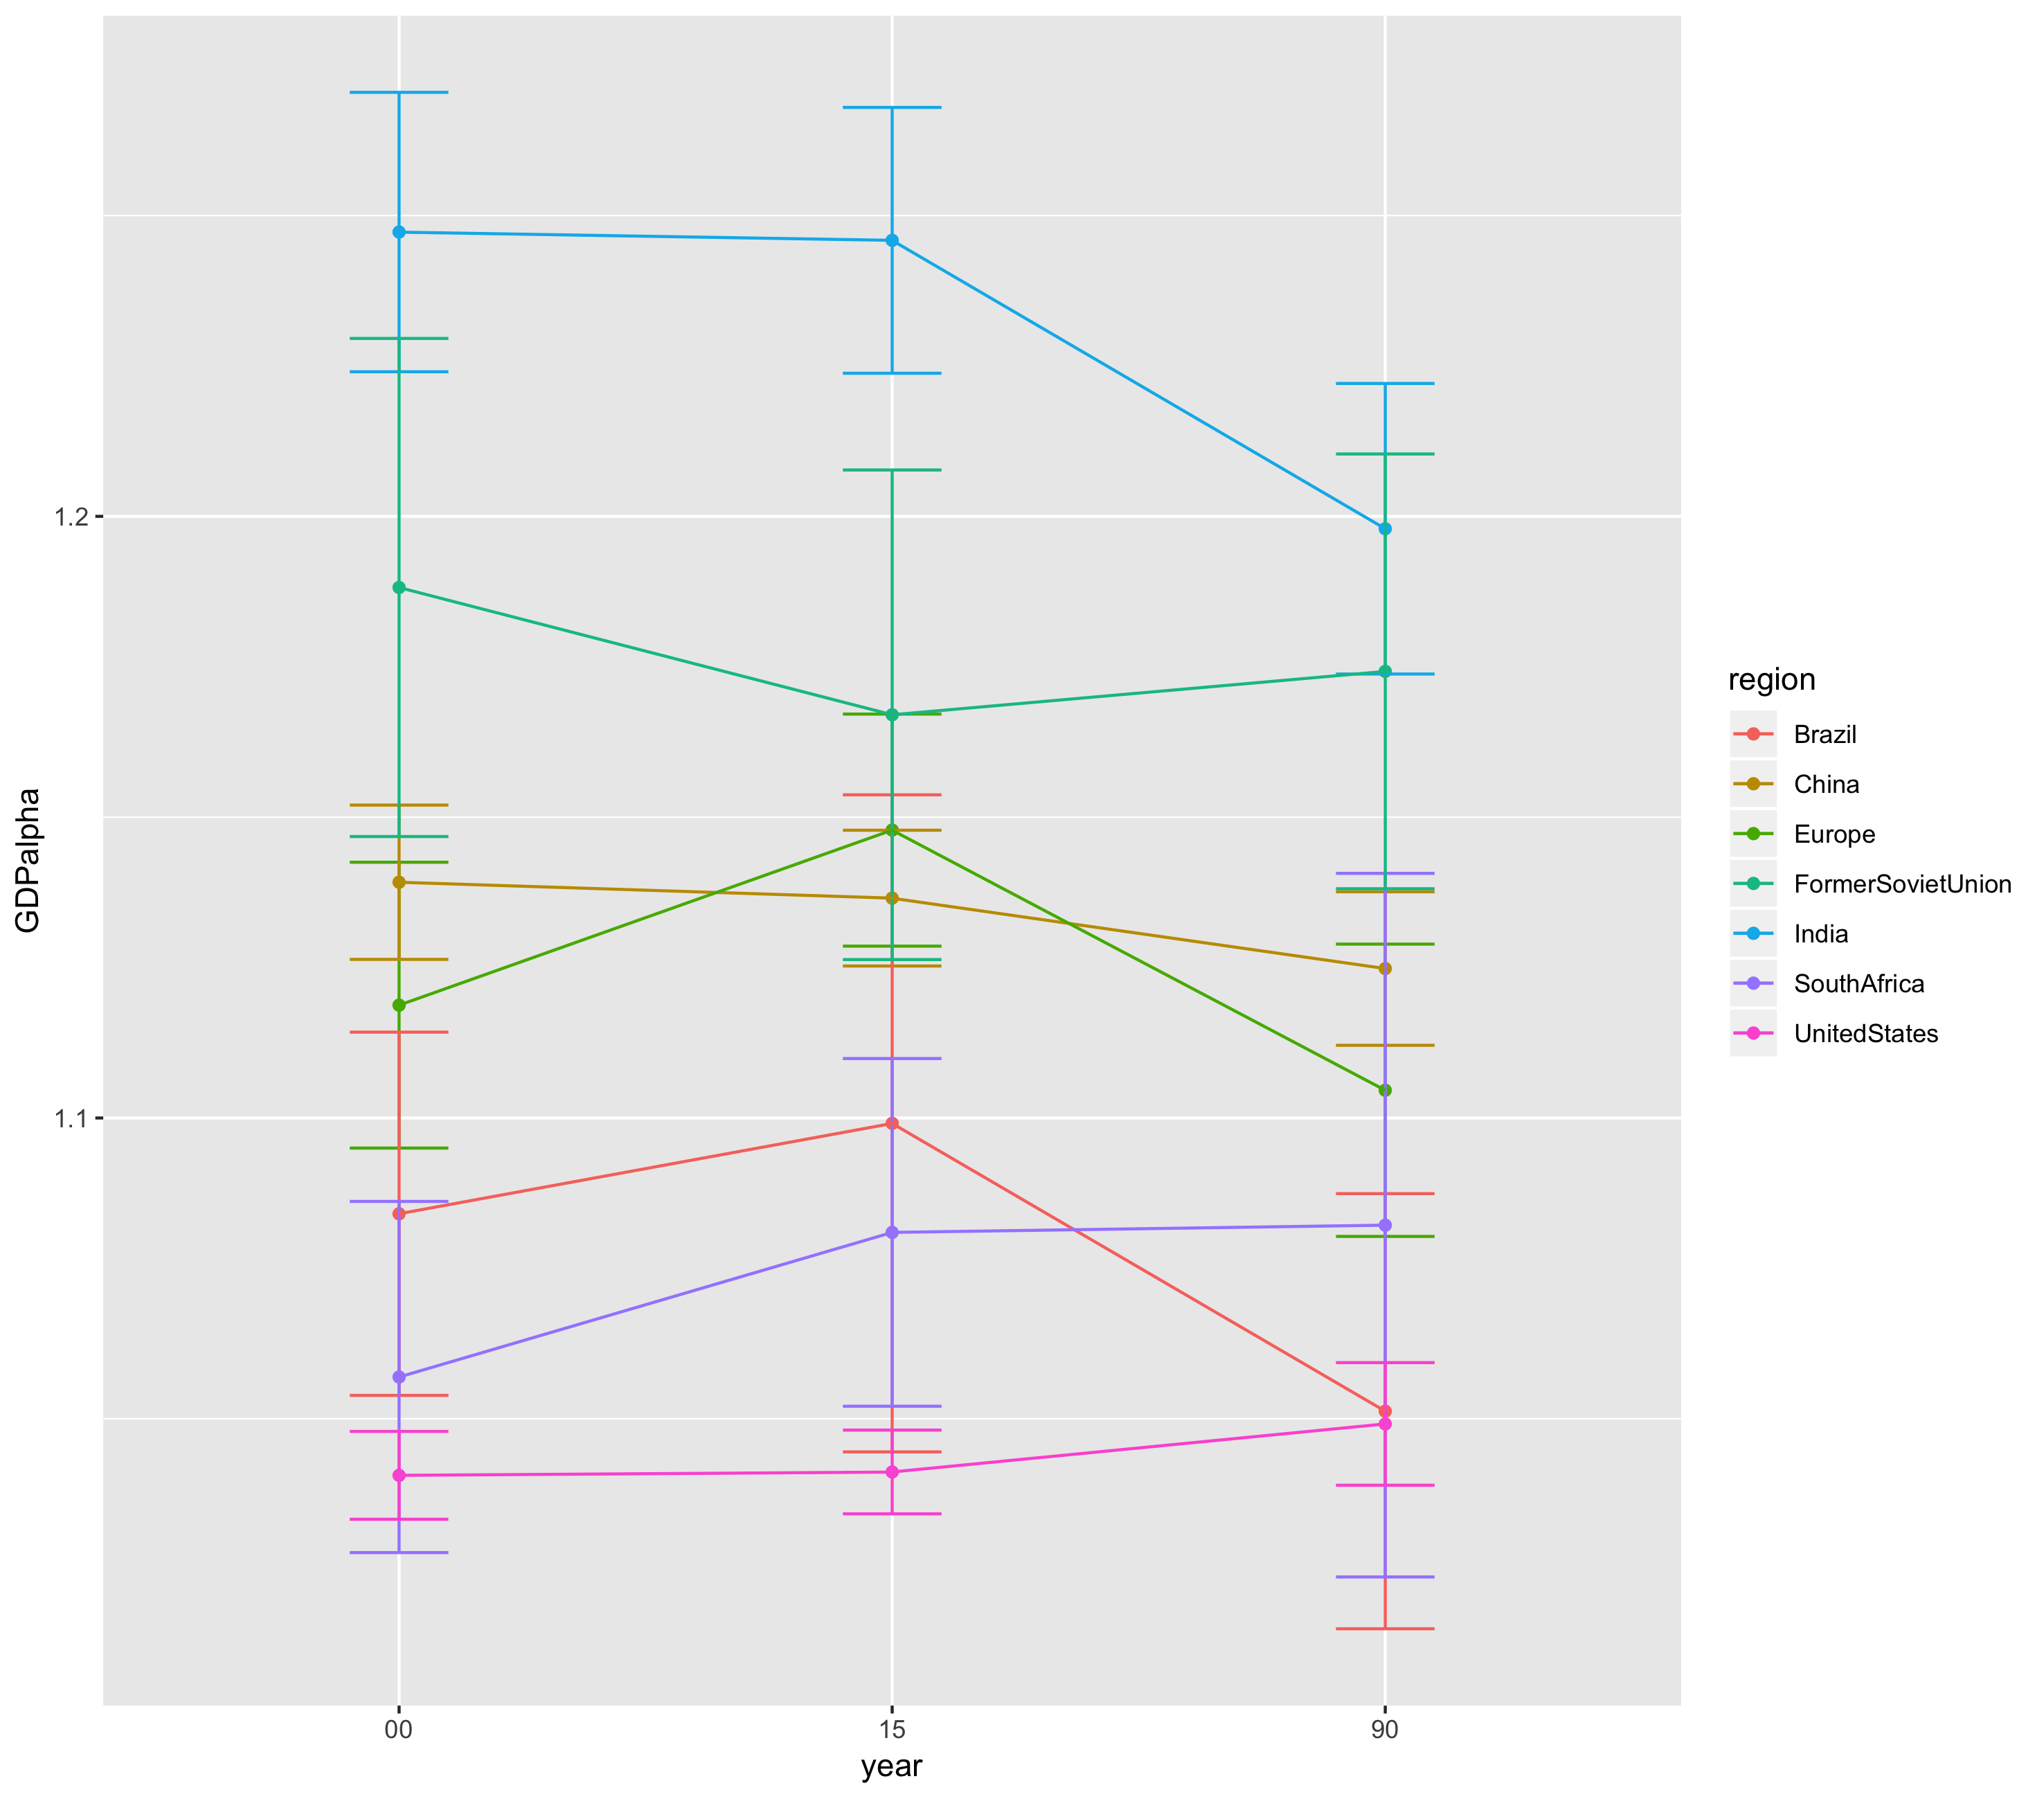
\includegraphics[width=0.32\textwidth,height=0.45\textheight]{figures/GDP-evolution_Europe-China-Brazil-India-SouthAfrica-UnitedStates-FormerSovietUnion_years-90-00-15.png}
\end{center}

}


\sframe{Summary of scaling exponents}{

}




\sframe{Fitting scaling laws}{

% \cite{finance2018absent}
% \cite{clauset2009power}
% \cite{leitao2016scaling}
% \cite{broido2019scale}
% \cite{smith2019biochemical}

% summary table of Goodness of fit for - classical scaling, with cutoff, as piecewise linear

\textit{Alternative models for better fit of scaling laws}


}


\sframe{Dynamical models of urban growth}{

}




\sframe{Discussion}{

% Open questions :
%  - urban scaling and dynamics
%  - endogenous areas for scaling and dynamical models ? 

}



%%%%%%%%%%%%%%%%%%%%%
\begin{frame}[allowframebreaks]
\frametitle{References}
\bibliographystyle{apalike}
\bibliography{biblio}
\end{frame}
%%%%%%%%%%%%%%%%%%%%%%%%%%%%










\end{document}




